	%%  A simple AAU report template.

%  2014-09-13 v. 1.1.0
%  Copyright 2010-2014 by Jesper Kjær Nielsen <jkn@es.aau.dk>
%
%  This is free software: you can redistribute it and/or modify
%  it under the terms of the GNU General Public License as published by
	%  the Free Software Foundation, either version 3 of the License, or
%  (at your option) any later version.
%
%  This is distributed in the hope that it will be useful,
%  but WITHOUT ANY WARRANTY; without even the implied warranty of
%  MERCHANTABILITY or FITNESS FOR A PARTICULAR PURPOSE.  See the
%  GNU General Public License for more details.
%
%  You can find the GNU General Public License at <http://www.gnu.org/licenses/>.
%
%  A simple AAU report template.
%  2014-09-13 v. 1.1.0
%  Copyright 2010-2014 by Jesper Kjær Nielsen <jkn@es.aau.dk>
%
%  This is free software: you can redistribute it and/or modify
%  it under the terms of the GNU General Public License as published by
%  the Free Software Foundation, either version 3 of the License, or
%  (at your option) any later version.
%
%  This is distributed in the hope that it will be useful,
%  but WITHOUT ANY WARRANTY; without even the implied warranty of
%  MERCHANTABILITY or FITNESS FOR A PARTICULAR PURPOSE.  See the
%  GNU General Public License for more details.
%
%  You can find the GNU General Public License at <http://www.gnu.org/licenses/>.
%
\documentclass[11pt,twoside,a4paper,openright]{report}
%%%%%%%%%%%%%%%%%%%%%%%%%%%%%%%%%%%%%%%%%%%%%%%%
% Language, Encoding and Fonts
% http://en.wikibooks.org/wiki/LaTeX/Internationalization
%%%%%%%%%%%%%%%%%%%%%%%%%%%%%%%%%%%%%%%%%%%%%%%%
% Select encoding of your inputs. Depends on
% your operating system and its default input
% encoding. Typically, you should use
%   Linux  : utf8 (most modern Linux distributions)
%            latin1 
%   Windows: ansinew
%            latin1 (works in most cases)
%   Mac    : applemac
% Notice that you can manually change the input
% encoding of your files by selecting "save as"
% an select the desired input encoding. 
\usepackage[utf8]{inputenc}
% Make latex understand and use the typographic
% rules of the language used in the document.
\usepackage[danish,english]{babel}
% Use the vector font Latin Modern which is going
% to be the default font in latex in the future.
\usepackage{lmodern}
% Choose the font encoding
\usepackage[T1]{fontenc}
% For checkmarks: \cmark and crossmarks: \xmark
\usepackage{pifont}
	\newcommand{\cmark}{\ding{51}}%
	\newcommand{\xmark}{\ding{55}}%
%%%%%%%%%%%%%%%%%%%%%%%%%%%%%%%%%%%%%%%%%%%%%%%%
% Graphics and Tables
% http://en.wikibooks.org/wiki/LaTeX/Importing_Graphics
% http://en.wikibooks.org/wiki/LaTeX/Tables
% http://en.wikibooks.org/wiki/LaTeX/Colors
%%%%%%%%%%%%%%%%%%%%%%%%%%%%%%%%%%%%%%%%%%%%%%%%
% load a colour package
\usepackage[table,dvipsnames]{xcolor}
\definecolor{aaublue}{RGB}{33,26,82}% dark blue
\definecolor{lightGrey}{RGB}{240,240,240}% 
\definecolor{Grey}{gray}{0.7}
% The standard graphics inclusion package
\usepackage{graphicx}
% Load package to convert eps-files to use as figures
\usepackage{epstopdf}

%\usepackage[dvips,final]{graphicx} 
%\usepackage[dvips]{geometry}
\usepackage{color,soul} %include even if images aren’t in color \usepackage{epsfig}
\usepackage{latexsym}
\usepackage{pstricks}

%\usepackage{epsfig}

% Set up how figure and table captions are displayed
\usepackage{caption}
\captionsetup{%
  font=footnotesize,% set font size to footnotesize
  labelfont=bf % bold label (e.g., Figure 3.2) font
}
\usepackage[section]{placeins} % Figurer overskrider ikke sections
% For subfigures
\usepackage{subcaption}
% Make the standard latex tables look so much better
\usepackage{array,booktabs}
% Enable the use of frames around, e.g., theorems
% The framed package is used in the example environment
\usepackage{framed}

% Afstand mellem listepunkter og tilføjelse af resume funktion til lister: \begin{enumerate}[resume]
\usepackage{enumitem}
\setlist{itemsep=-2pt}

% Tilføjer mulighed for at lave enkelte sider i landskab.
\usepackage{lscape}

\newcounter{listcounter}
%%%%%%%%%%%%%%%%%%%%%%%%%%%%%%%%%%%%%%%%%%%%%%%%
% Mathematics
% http://en.wikibooks.org/wiki/LaTeX/Mathematics
%%%%%%%%%%%%%%%%%%%%%%%%%%%%%%%%%%%%%%%%%%%%%%%%
% Defines new environments such as equation,
% align and split 
\usepackage{amsmath}
% Adds new math symbols
\usepackage{amssymb}
% Use theorems in your document
% The ntheorem package is also used for the example environment
% When using thmmarks, amsmath must be an option as well. Otherwise \eqref doesn't work anymore.
\usepackage[framed,amsmath,thmmarks]{ntheorem}

% Tilføjer \degree symbol
\usepackage{textcomp}
\usepackage{gensymb}

% Fjerner mellemrum efter komma i formler.
%\usepackage{icomma}

% Packages for SI units
\usepackage[binary-units]{siunitx}
% Format SI units as italic in italic texts
\sisetup{detect-all}
\sisetup{per-mode=symbol}


% Argument til amsmath der gør parenteser uden om parenteser pænere ved brug af \right og \left kommandoerne
\delimitershortfall=-1pt

%%%%%%%%%%%%%%%%%%%%%%%%%%%%%%%%%%%%%%%%%%%%%%%%
% Page Layout
% http://en.wikibooks.org/wiki/LaTeX/Page_Layout
%%%%%%%%%%%%%%%%%%%%%%%%%%%%%%%%%%%%%%%%%%%%%%%%
% Change margins, papersize, etc of the document
\usepackage[
  inner=28mm,% left margin on an odd page
  outer=41mm,% right margin on an odd page
  ]{geometry}
% Modify how \chapter, \section, etc. look
% The titlesec package is very configureable
\usepackage[explicit]{titlesec}
%\titleformat*{\section}{\normalfont\Large\bfseries\color{aaublue}}
%\titleformat*{\subsection}{\normalfont\large\bfseries\color{aaublue}}
%\titleformat*{\subsubsection}{\normalfont\normalsize\bfseries\color{aaublue}}
%\titleformat*{\paragraph}{\normalfont\normalsize\bfseries\color{aaublue}}
%\titleformat*{\subparagraph}{\normalfont\normalsize\bfseries\color{aaublue}}
\usepackage{calc}

% Spacing omkring kapiteloverskrift
\titlespacing*{\chapter}{0pt}{40pt}{50pt}



% Overskrift med stort nummer til venstre og titel til højre
%\newlength\chapnumb
%\setlength{\chapnumb}{1.5cm}
%\titleformat{\chapter}[block]
%{\normalfont\bfseries}{}{0pt}
%{\parbox[b]{\chapnumb}{%
	  %\fontsize{2cm}{0}\selectfont\thechapter}%
  %\parbox[b]{\dimexpr\textwidth-\chapnumb\relax}{%
    %\raggedleft%
    %\hfill{\Huge#1}\\
    %\rule{\dimexpr\textwidth-\chapnumb\relax}{.5pt}}}
%\titleformat{name=\chapter,numberless}[block]
%{\normalfont\bfseries}{}{0pt}
	%{\Huge#1}

% Clear empty pages between chapters
\let\origdoublepage\cleardoublepage
\newcommand{\clearemptydoublepage}{%
  \clearpage
  {\pagestyle{empty}\origdoublepage}%
}
\let\cleardoublepage\clearemptydoublepage

% Change the headers and footers
\usepackage{fancyhdr}
\pagestyle{fancy}
\fancyhf{} %delete everything
\renewcommand{\headrulewidth}{0pt} %remove the horizontal line in the header
\fancyhead[RE]{\color{black}\small\nouppercase\leftmark} %even page - chapter title
\fancyhead[LO]{\color{black}\small\nouppercase\rightmark} %uneven page - section title
\fancyhead[LE,RO]{\thepage} %page number on all pages
% Do not stretch the content of a page. Instead,
% insert white space at the bottom of the page
\raggedbottom
% Enable arithmetics with length. Useful when
% typesetting the layout.

\setlength{\headheight}{14pt}

% Raise penalties for bastards
\widowpenalty=10000
\clubpenalty=10000

%%%%%%%%%%%%%%%%%%%%%%%%%%%%%%%%%%%%%%%%%%%%%%%%
% Table of Contents
% http://en.wikibooks.org/wiki/LaTeX/Bibliography_Management
%%%%%%%%%%%%%%%%%%%%%%%%%%%%%%%%%%%%%%%%%%%%%%%%
% Add additional commands for Table of Contents
\usepackage{bookmark}

{\setcounter{tocdepth}{1}}

% Control of space between items in Table of Contents
\usepackage[titles]{tocloft}
\setlength{\cftbeforepartskip}{10pt}
\setlength{\cftbeforechapskip}{4pt}
\setlength{\cftbeforesecskip}{2pt}
%%%%%%%%%%%%%%%%%%%%%%%%%%%%%%%%%%%%%%%%%%%%%%%%
% Bibliography
% http://en.wikibooks.org/wiki/LaTeX/Bibliography_Management
%%%%%%%%%%%%%%%%%%%%%%%%%%%%%%%%%%%%%%%%%%%%%%%%
% Add the \citep{key} command which display a
% reference as [author, year]
\usepackage[square]{natbib}

%%%%%%%%%%%%%%%%%%%%%%%%%%%%%%%%%%%%%%%%%%%%%%%%
% Misc
%%%%%%%%%%%%%%%%%%%%%%%%%%%%%%%%%%%%%%%%%%%%%%%%
% Add bibliography and index to the table of
% contents
\usepackage[nottoc]{tocbibind}
% Add the command \pageref{LastPage} which refers to the
% page number of the last page
\usepackage{lastpage}
\usepackage[
%  disable, %turn off todonotes
  colorinlistoftodos, %enable a coloured square in the list of todos
  textwidth=\marginparwidth, %set the width of the todonotes
  textsize=scriptsize, %size of the text in the todonotes
  ]{todonotes}

% Add command \includepdf to add a whole pdf page to document
\usepackage{pdfpages}


% Add option to easy format directory tree
\usepackage{dirtree}

% String manipulation
\usepackage{xstring,xifthen}

% Tikz package for drawing nice figures
\usepackage{tikz}
\usepackage{schemabloc}
\usetikzlibrary{circuits}


% Package for drawing pretty schematics, without leaving LaTex
\usepackage[american currents, american voltages, european resistors, cute inductors,
american ports]{circuitikz}
\usepackage{tikzscale}

% Code syntax highlight
\usepackage{listings}
\lstset{breaklines=true,
		breakatwhitespace=true,
		commentstyle=\color{ForestGreen},
		numbers=left,
		numberstyle=\tiny\color{black},
		keywordstyle=\color{blue},
		basicstyle=\footnotesize\ttfamily,
        showstringspaces=false,
		}
\renewcommand{\lstlistingname}{Code Snippet}

%%%%%%%%%%%%%%%%%%%%%%%%%%%%%%%%%%%%%%%%%%%%%%%%
% Table environments
% http://en.wikibooks.org/wiki/LaTeX/Tables
%%%%%%%%%%%%%%%%%%%%%%%%%%%%%%%%%%%%%%%%%%%%%%%%
% Better table environments for stuff like table width specifier
\usepackage{tabularx}
\usepackage{multirow}
\usepackage{longtable}
\usepackage{makecell}
%%%%%%%%%%%%%%%%%%%%%%%%%%%%%%%%%%%%%%%%%%%%%%%%
% Project info and abstract
% chapters\abstract.tex, chapters\projectinfo.tex
%%%%%%%%%%%%%%%%%%%%%%%%%%%%%%%%%%%%%%%%%%%%%%%%
% Loads project info and abstract for use in
% hypersetup
\newcommand{\projectFaculty}{%
\iflanguage{english}{%
Vision, Graphics and Interactive Systems%
}{%
Vision, Grafik og Interaktive Systemer%
}}

\newcommand{\projectGroup}{%
\iflanguage{english}{%
Group 18gr942%
}{%
Gruppe 18gr942%
}}

\newcommand{\projectSemester}{%
P8%
}

\newcommand{\projectType}{%
\iflanguage{english}{%
Project Report%
}{%
Projektrapport%
}}

\newcommand{\projectTitle}{%
\iflanguage{english}{%
AIVERO AS Internship%
}{%
Noget med Computer Vision%
}}

\newcommand{\projectSubtitle}{%
\iflanguage{english}{%
- Subtitle -%
}{%
- Undertitel -%
}}

\newcommand{\projectTheme}{%
\iflanguage{english}{%
Computer Vision%
}{%
Computer Vision%
}}

\newcommand{\projectPeriod}{%
\iflanguage{english}{%
Fall Semester 2018%
}{%
Forårssemester 2018%
}}



\newcommand{\projectParticipants}{%
Niclas Hjorth Stjernholm
}

\newcommand{\projectSupervisors}{%
Thomas B. Moeslund\\
Raphael Düershceid
}

\newcommand{\projectCopies}{8}

\newcommand{\projectCompletion}{
\iflanguage{english}{%
January 9, 2019%
}{
30. maj 2018%
}}

\newcommand{\projectAbstract}{

}

\newcommand{\projectSynopsis}{
Synopsis
}


%%%%%%%%%%%%%%%%%%%%%%%%%%%%%%%%%%%%%%%%%%%%%%%%
% Hyperlinks
% http://en.wikibooks.org/wiki/LaTeX/Hyperlinks
%%%%%%%%%%%%%%%%%%%%%%%%%%%%%%%%%%%%%%%%%%%%%%%%
% Enable hyperlinks and insert info into the pdf
% file. Hypperref should be loaded as one of the 
% last packages
\usepackage{hyperref}
\hypersetup{%
	%pdfpagelabels=true,%
	plainpages=false,%
	pdfauthor={\projectGroup, \projectFaculty, \iflanguage{english}{Aalborg University}{Aalborg Universitet}},%
	pdftitle={\projectTitle},%
	pdfsubject={\projectTheme},%
	bookmarksnumbered=true,%
	colorlinks,%
	citecolor=black,%aaublue,%
	filecolor=black,%aaublue,%
	linkcolor=black,%aaublue,% you should probably change this to black before printing
	urlcolor=black,%aaublue,%
	pdfstartview=FitH,%
	bookmarksdepth=2,%
}

% Defines where URLs should break
\def\UrlBreaks{\do\/\do-\do_}
\urlstyle{same}

% Give the possibility to autoformat reference based on distance to the referenced page. Ex. \vpageref{}
\usepackage{varioref}


% Package to warn about missing references.
%\usepackage{refcheck}

% Package to make a glossary of acronyms.
\usepackage[nonumberlist]{glossaries}
\usepackage{glossary-mcols}
\glstoctrue
\makenoidxglossaries
\glssetwidest{DeepID2  }
\glossarystyle{alttree}
% Glossaries package
% http://ctan.cs.uu.nl/macros/latex/contrib/glossaries/glossariesbegin.pdf
%
% % % % % % % %
%	Example of glossary entry:
% \newglossaryentry{cabbage}{name={cabbage},description={vegetable with thick green or purple leaves}}
%
%	Example of acronym entry:
% \newacronym{spi}{SPI}{Serial Peripheral Interface}
%
% \gls{key}

\newacronym{cdf}{CDF}{Cumulative Distribution Function}
\newacronym{cnn}{CNN}{Convolutional Neural Network}
\newacronym{cpu}{CPU}{Central Processing Unit}
\newacronym{fcn}{FCN}{Fully Convolutional Network}
\newacronym{dbn}{DBN}{Deep Belief Network}
\newacronym{deepid}{DeepID}{Deep hidden identity features}
\newacronym{deepid2}{DeepID2}{Deep IDentification-verification features}
\newacronym{gpu}{GPU}{Graphics Processing Unit}
\newacronym{spdnn}{SPDNN}{Semi Parallel Deep Neural Networks}
\newacronym{lfw}{LFW}{Labeled Faces in the Wild}
\newacronym{hmm}{HMM}{Hidden Markov Model}
\newacronym{lda}{LDA}{Linear Discriminant Analysis}
\newacronym{pca}{PCA}{Principal Component Analysis}
\newacronym{svm}{SVM}{support vector machines}
\newacronym{knn}{KNN}{K-Nearest-Neighbours}
\newacronym{vl}{VL}{Visible Light}
\newacronym{nir}{NIR}{Near Infra-Red}
\newacronym{mcs}{MCS}{Multiple Classifier Systems}
\newacronym{relu}{ReLU}{Rectified Linear Unit}
\newacronym{fc}{FC}{Fully Connected}
\newacronym{yolo}{YOLO}{You Only Look Once}
\newacronym{mot}{MOT}{Multiple Object Tracking benchmark}
\newacronym{gqcnn}{GQ-CNN}{Grasp Quality Convolutional Neural Network}
\newacronym{rgbd}{RGB-D}{Red, Green, Blue, Depth}
\newacronym{dof}{DOF}{Degrees of Freedom}
\newacronym{fps}{FPS}{Frames per Second}
\newacronym{gstapp}{GStAPP}{GStreamer application}


% Package to make semi-bold font.
\usepackage[outline]{contour}
\contourlength{0.1pt}
\contournumber{50}%
\newcommand{\textsb}[1]{\contour{black}{#1}}

% Package for splitting lists or other things up in columns. Ex: \begin{multicols}{2}
\usepackage{multicol}

% Package for rotating a page to landscape orientation. Ex: \begin{landscape}
\usepackage{pdflscape}

% Package for circuit diagrams in tikz
\usepackage{circuitikz}

% For adding notes to tables
\usepackage{threeparttable}

% For adding smileys ;) I know....
\usepackage{MnSymbol,wasysym}

% For adding algorithms
\usepackage{algorithm}
\usepackage[noend]{algpseudocode}
\makeatletter
\def\BState{\State\hskip-\ALG@thistlm}
\makeatother

\renewcommand*{\glsgroupskip}{\vspace{2mm}}

% Package to use fixme fxnote
\usepackage[footnote,marginclue,draft,danish,silent,nomargin]{fixme} 

% Package inclusion and set up of the document

% see, e.g., http://en.wikibooks.org/wiki/LaTeX/Formatting#Hyphenation
% for more information on word hyphenation
\hyphenation{ex-am-ple hy-phen-a-tion short}
\hyphenation{long la-tex}
\hyphenation{AAU-Sat}
\hyphenation{minimum-spændinger}
\hyphenation{ud-vik-lings-poten-tiale}
\hyphenation{pick-up pick-up-pen gui-tar-pick-up gui-tar-pick-up-pen pick-uppens}
\hyphenation{tech-no-lo-gy}
\hyphenation{Hø-re-for-e-ning-en}
\hyphenation{dis-cri-mi-nant}% Hypenation setup

%  A simple AAU report template.
%  2014-09-13 v. 1.1.0
%  Copyright 2010-2014 by Jesper Kjær Nielsen <jkn@es.aau.dk>
%
%  This is free software: you can redistribute it and/or modify
%  it under the terms of the GNU General Public License as published by
%  the Free Software Foundation, either version 3 of the License, or
%  (at your option) any later version.
%
%  This is distributed in the hope that it will be useful,
%  but WITHOUT ANY WARRANTY; without even the implied warranty of
%  MERCHANTABILITY or FITNESS FOR A PARTICULAR PURPOSE.  See the
%  GNU General Public License for more details.
%
%  You can find the GNU General Public License at <http://www.gnu.org/licenses/>.
%
%
%
% see, e.g., http://en.wikibooks.org/wiki/LaTeX/Customizing_LaTeX#New_commands
% for more information on how to create macros

%%%%%%%%%%%%%%%%%%%%%%%%%%%%%%%%%%%%%%%%%%%%%%%%
% Loads user defined variables
%%%%%%%%%%%%%%%%%%%%%%%%%%%%%%%%%%%%%%%%%%%%%%%%

\newcommand{\noSIunit}{$1$}% Definerer hvad der skal skrives hvis symbolet ikke har nogen enhed.
\newcommand{\obcTransducerAddress}{0xB1}% CAN adresse til tranducer modulet i OBC.

\def\circuitScale{.5}%

%%%%%%%%%%%%%%%%%%%%%%%%%%%%%%%%%%%%%%%%%%%%%%%%
% Macros for the titlepage
%%%%%%%%%%%%%%%%%%%%%%%%%%%%%%%%%%%%%%%%%%%%%%%%
%Creates the aau titlepage
\newcommand{\aautitlepage}[3]{%
  {
    %set up various length
    \ifx\titlepageleftcolumnwidth\undefined
      \newlength{\titlepageleftcolumnwidth}
      \newlength{\titlepagerightcolumnwidth}
    \fi
    \setlength{\titlepageleftcolumnwidth}{0.5\textwidth-\tabcolsep}
    \setlength{\titlepagerightcolumnwidth}{\textwidth-2\tabcolsep-\titlepageleftcolumnwidth}
    %create title page
    \thispagestyle{empty}
    \noindent%
    \begin{tabular}{@{}ll@{}}
      \parbox{\titlepageleftcolumnwidth}{
        \iflanguage{danish}{%
          
\includegraphics[page=1,width=\titlepageleftcolumnwidth]{figures/aau_logo}
        }{%
          
\includegraphics[page=2,width=\titlepageleftcolumnwidth]{figures/aau_logo}
        }
      } &
      \parbox{\titlepagerightcolumnwidth}{\raggedleft\sf\small
        #2
      }\bigskip\\
       #1 &
      \parbox[t]{\titlepagerightcolumnwidth}{%
        \iflanguage{danish}{%
          \textbf{Synopsis:}\smallskip\par
        }{%
          \textbf{Abstract:}\smallskip\par
        }
        \fbox{\parbox{\titlepagerightcolumnwidth-2\fboxsep-2\fboxrule}{%
          #3
        }}
      }\\
    \end{tabular}
    \vfill
    \iflanguage{danish}{%
      \noindent{\footnotesize\emph{Rapportens indhold er frit tilgængeligt, men offentliggørelse (med kildeangivelse) må kun ske efter aftale med forfatterne.}}
    }{%
      \noindent{\footnotesize\emph{The content of this report is freely available, but publication may only be pursued with reference.}}
    }
    \cleardoublepage
  }
}

%Create english project info
\newcommand{\englishprojectinfo}[8]{%
  \parbox[t]{\titlepageleftcolumnwidth}{
    \textbf{Title:}\\ #1\bigskip\par
    \textbf{Theme:}\\ #2\bigskip\par
    \textbf{Project Period:}\\ #3\bigskip\par
    \textbf{Project Group:}\\ #4\bigskip\par
    \textbf{Participants:}\\ #5\bigskip\par
    \textbf{Supervisor:}\\ #6\bigskip\par
    \textbf{Number of Pages:} \pageref{LastPage}\bigskip\par
    \textbf{Date of Completion:}\\ #8
  }
}

%Create danish project info
\newcommand{\danishprojectinfo}[8]{%
  \parbox[t]{\titlepageleftcolumnwidth}{
    \textbf{Titel:}\\ #1\bigskip\par
    \textbf{Tema:}\\ #2\bigskip\par
    \textbf{Projektperiode:}\\ #3\bigskip\par
    \textbf{Projektgruppe:}\\ #4\bigskip\par
    \textbf{Deltagere:}\\ #5\bigskip\par
    \textbf{Vejleder:}\\ #6\bigskip\par
    \textbf{Oplagstal:} #7\bigskip\par
    \textbf{Sidetal:} \pageref{LastPage}\bigskip\par
    \textbf{Afleveringsdato:}\\ #8
  }
}

%%%%%%%%%%%%%%%%%%%%%%%%%%%%%%%%%%%%%%%%%%%%%%%%
% An example environment
%%%%%%%%%%%%%%%%%%%%%%%%%%%%%%%%%%%%%%%%%%%%%%%%
\theoremheaderfont{\normalfont\bfseries}
\theorembodyfont{\normalfont}
\theoremstyle{break}
\def\theoremframecommand{{\color{aaublue!50}\vrule width 5pt \hspace{5pt}}}
\newshadedtheorem{exa}{Example}[chapter]
\newenvironment{example}[1]{%
		\begin{exa}[#1]
}{%
		\end{exa}
}


%%%%%%%%%%%%%%%%%%%%%%%%%%%%%%%%%%%%%%%%%%%%%%%%%
% Exponential function defined as upright e, \exp
%%%%%%%%%%%%%%%%%%%%%%%%%%%%%%%%%%%%%%%%%%%%%%%%%
\renewcommand{\exp}{\text{e}}


%%%%%%%%%%%%%%%%%%%%%%%%%%%%%%%%%%%%%%%%%%%%%%%%%%%
% Command \clearevenpage start chapter on even page
%%%%%%%%%%%%%%%%%%%%%%%%%%%%%%%%%%%%%%%%%%%%%%%%%%%
\makeatletter
\newcommand*{\clearevenpage}{%
  \clearpage
  \if@twoside
    \ifodd\c@page
      \hbox{}%
      \newpage
      \if@twocolumn
        \hbox{}%
        \newpage
      \fi
    \fi
  \fi
}
\makeatother

%%%%%%%%%%%%%%%%%%%%%%%%%%%%%%%%%%%%%%%%%%%%%%%%%%%%%%%
% Command \addunit. Use it to add si units to equations
%%%%%%%%%%%%%%%%%%%%%%%%%%%%%%%%%%%%%%%%%%%%%%%%%%%%%%%
\makeatletter
\providecommand\add@text{}
\newcommand\addunit[1]{%
  \gdef\add@text{\text{[}\ifthenelse{\equal{#1}{}}{\noSIunit}{\si{#1}}\text{]}\gdef\add@text{}}}% 
\renewcommand\tagform@[1]{%
  \maketag@@@{\llap{\add@text\quad}(\ignorespaces#1\unskip\@@italiccorr)}%
}
\makeatother

%%%%%%%%%%%%%%%%%%%%%%%%%%%%%%%%%%%%%%%%%%%%%
% Oversættelser af ord ved brug af \autoref{}
%%%%%%%%%%%%%%%%%%%%%%%%%%%%%%%%%%%%%%%%%%%%%
\addto\extrasdanish{%
  \def\figureautorefname{Figur}%
  \def\subfigureautorefname{Figur}%
  \def\tableautorefname{Tabel}%
  \def\partautorefname{Del}%
  \def\appendixautorefname{Bilag}%
  \def\equationautorefname{Ligning}%
  \def\Itemautorefname{Punkt}%
  \def\chapterautorefname{Kapitel}%
  \def\sectionautorefname{Afsnit}%
  \def\subsectionautorefname{Afsnit}%
  \def\subsubsectionautorefname{Underafsnit}%
  \def\paragraphautorefname{Delafsnit}%
  \def\Hfootnoteautorefname{Fodnote}%
  \def\AMSautorefname{Ligning}%
  \def\theoremautorefname{Sætning}%
  \def\pageautorefname{Side}%
  \def\requirementautorefname{Krav}%
}

\addto\extrasenglish{%
  \def\sectionautorefname{section}%
  \def\subsectionautorefname{section}%
  \def\subsubsectionautorefname{section}%
  \def\requirementautorefname{Requirement}%
  \def\algorithmautorefname{Algorithm}%
}

%%%%%%%%%%%%%%%%%%%%%%%%%%%%%%%%%%%%%%%%%%%%%%%%%%%%%%%%%%%%%%%%%%%%%%
% Tilføjer kommando \fullref{} for både at referere til nummer og navn
%%%%%%%%%%%%%%%%%%%%%%%%%%%%%%%%%%%%%%%%%%%%%%%%%%%%%%%%%%%%%%%%%%%%%%
\renewcommand*{\fullref}[1]{\hyperref[{#1}]{\autoref*{#1} \nameref*{#1}}} % One single link


%%%%%%%%%%%%%%%%%%%%%%%%%%%%%%%%%%%%%%%%%%%%%%%%%%%%%%%%%%%%%%%%%%%%%%
% Tilføjer forkortelser af ord.
%%%%%%%%%%%%%%%%%%%%%%%%%%%%%%%%%%%%%%%%%%%%%%%%%%%%%%%%%%%%%%%%%%%%%%
\newcommand{\AAU}{%
\iflanguage{english}{%
Aalborg University%
}{%
Aalborg Universitet%
}}

\newcommand{\opamp}{%
\iflanguage{english}{%
operational amplifier%
}{%
operationsforstærker%
}}

\newcommand{\hifi}{%
\iflanguage{english}{%
hi-fi amplifier%
}{%
hi-fi-forstærker%
}}

%%%%%%%%%%%%%%%%%%%%%%%%%%%%%%%%%%%%%%%%%%%%%%%%%%%%%%%%%%%%%%%%%%%%%%
% Command \DefVar{VARIBLE_NAME}
% Is used to create a variable.
% Set varible: \VARIBLE_NAME{VALUE}
% Get varible: \getVARIBLE_NAME
%%%%%%%%%%%%%%%%%%%%%%%%%%%%%%%%%%%%%%%%%%%%%%%%%%%%%%%%%%%%%%%%%%%%%%

\makeatletter%
\newcommand{\DefVar}[1]{\@namedef{#1}##1{\global\@namedef{get#1}{##1}}\@nameuse{#1}{}}%
\makeatother%

%%%%%%%%%%%%%%%%%%%%%%%%%%%%%%%%%%%%%%%%%%%%%%%%%%%%%%%%%%%%%%%%%%%%%%
% Requirements environment:
%
% \begin{requirement}
%   \requirement{}
%   \argument{}
%   \fullfilment{}
% \end{requirement}
%%%%%%%%%%%%%%%%%%%%%%%%%%%%%%%%%%%%%%%%%%%%%%%%%%%%%%%%%%%%%%%%%%%%%%

\def\reqPrefixName{??}% Individual prefix for the requirements
\newcounter{reqIDCounter}% Requirement counter for the subsections
\newcounter{requirement}% Absolute requirement counter. Used to trigger label/reference target.

\newlength{\reqBoxWidth}% Create length varible to define width of requirement box
\setlength{\reqBoxWidth}{5cm}% Actual width of requirement box

\newcommand{\reqPrefix}[1]{% Command to define requirement prefix
\ifthenelse{\equal{#1}{}}{\reqPrefixName}{\setcounter{reqIDCounter}{0}\def\reqPrefixName{#1}}%
}

\makeatletter% Define requirementID for references
\newcommand{\reqLabel}{%
\protected@edef\@currentlabel{\reqPrefixName\thereqIDCounter}%
\protected@edef\@currentlabelname{Requirement}%
}\makeatother%

\newenvironment{requirement}%
{\par\vspace{\baselineskip}\noindent\ignorespaces%
\refstepcounter{requirement}%
\stepcounter{reqIDCounter}%
\reqLabel%
\DefVar{requirement}\DefVar{argument}\DefVar{fullfilment}%
%
\tabularx{1\textwidth}{p{\reqBoxWidth} !{\color{white}{\vrule width 2pt}} X}%
\greyrow \parbox[t]{\reqBoxWidth}{\textsb{Requirement~\reqPrefixName\thereqIDCounter}\\\getrequirement\vskip1mm}%
&%
\parbox[t]{\textwidth-\reqBoxWidth-4\tabcolsep-2pt}{\textsb{Argumentation}\\\getargument\vskip1mm}\\
\addlinespace[2pt]%
\greyrow \multicolumn{2}{l}{\parbox{\textwidth-2\tabcolsep}{\vskip1mm\textsb{Conditions of fulfilment}\\\getfullfilment\vskip1mm}}%
}%
{\endtabularx\par\ignorespacesafterend}


%%%%%%%%%%%%%%%%%%%%%%%%%%%%%%%%%%%%%%%%%%%%%%%%%%%%%%%%%%%%%%%%%%%%%%
% Tilføjer kommando \numnameref{labelnavn}
% Kommandoen tilføjer en reference til et afsnit med både nummer og navn.
%%%%%%%%%%%%%%%%%%%%%%%%%%%%%%%%%%%%%%%%%%%%%%%%%%%%%%%%%%%%%%%%%%%%%%
\newcommand{\numnameref}[1]{%
\hyperref[#1]{\autoref{#1}: \nameref{#1}}%
}

%%%%%%%%%%%%%%%%%%%%%%%%%%%%%%%%%%%%%%%%%%%%%%%%%%%%%%%%%%%%%%%%%%%%%%
% Defines subscript as upright text if it contains more than one character.
% 
%%%%%%%%%%%%%%%%%%%%%%%%%%%%%%%%%%%%%%%%%%%%%%%%%%%%%%%%%%%%%%%%%%%%%%

\catcode`\_=12% Makes underscore an inactive character
\begingroup\lccode`~=`\_% Loads underscore character for redefinition
\lowercase{\endgroup\def~}#1{% Start definition of underscore
\StrLen{#1}[\subscriptstringlen]% Determine length of subscript string
\ifthenelse{\subscriptstringlen=1}% Test if subscript string contain one character
{\sb{#1}}% Prints subscript as italic if only one character is present
{\sb{\mathrm{#1}}}}% Prints subscript as upright text if there are more than one character
\AtBeginDocument{\mathcode`\_=\string"8000 }% Makes underscore active only in math mode



%%%%%%%%%%%%%%%%%%%%%%%%%%%%%%%%%%%%%%%%%%%%%%%%%%%%%%%%%%%%%%%%%%%%%%
% Tilføjer kommando \startexplain, \stopexplain og \explain{}{}
% Bruges til forklaringer af ligninger.
%%%%%%%%%%%%%%%%%%%%%%%%%%%%%%%%%%%%%%%%%%%%%%%%%%%%%%%%%%%%%%%%%%%%%%
\newcounter{firstexplain}% Holder styr på om det er den første symbolforklaring

\def\startexplain{%
	\setcounter{firstexplain}{1}%
	{\noindent}%
	{\par\noindent}
	\begin{tabular}{@{}p{.06\columnwidth}p{.76\columnwidth}@{\hskip.04\columnwidth}p{.02\columnwidth}@{}}}%
\def\stopexplain{\end{tabular}\\[10pt]}%

\newcommand{\explain}[2]{%
	\ifthenelse{\thefirstexplain=1}{%
	Where:\\
	&#1&[\ifthenelse{\equal{#2}{}}{\noSIunit}{#2}]\\\setcounter{firstexplain}{0}
	}{%
	&#1&[\ifthenelse{\equal{#2}{}}{\noSIunit}{#2}]\\%
	}%
}%

%%%%%%%%%%%%%%%%%%%%%%%%%%%%%%%%%%%%%%%%%%%%%%%%%%%%%%%%%%%%%%%%%%%%%%
% Tilføjer kommando \startexplain, \stopexplain og \explain{}{}
% Bruges til forklaringer af ligninger.
%%%%%%%%%%%%%%%%%%%%%%%%%%%%%%%%%%%%%%%%%%%%%%%%%%%%%%%%%%%%%%%%%%%%%%





%%%%%%%%%%%%%%%%%%%%%%%%%%%%%%%%%%%%%%%%%%%%%%%%%%%%%%%%%%%%%%%%%%%%%%
% Tilføjer kommando \hyph
% Bruges til bindestreger i ord så de stadig kan deles korrekt af Latex.
%%%%%%%%%%%%%%%%%%%%%%%%%%%%%%%%%%%%%%%%%%%%%%%%%%%%%%%%%%%%%%%%%%%%%%
\def\hyph{-\penalty0\hskip0pt\relax}


%%%%%%%%%%%%%%%%%%%%%%%%%%%%%%%%%%%%%%%%%%%%%%%%%%%%%%%%%%%%%%%%%%%%%%
% Tilføjer kommando \hex og \bin
% Bruges til at skrive hexidecimal og binære tal.
%%%%%%%%%%%%%%%%%%%%%%%%%%%%%%%%%%%%%%%%%%%%%%%%%%%%%%%%%%%%%%%%%%%%%%
\newcommand{\hex}[1]{%
	\texttt{#1$_{16}$}
}%

\newcommand{\bin}[1]{%
	\texttt{#1$_{2}$}
}%


\newcommand{\greyrow}{%
	\rowcolor{lightGrey}
}%


%%%%%%%%%%%%%%%%%%%%%%%%%%%%%%%%%%%%%%%%%%%%%%%%%%%%%%%%%%%%%%%%%%%%%%
% Tilføjer kommando \citeref
% Bruges til at referere til egen rapport/bilag.
%%%%%%%%%%%%%%%%%%%%%%%%%%%%%%%%%%%%%%%%%%%%%%%%%%%%%%%%%%%%%%%%%%%%%%
\newcommand{\citeref}[1]{%
	[\autoref{#1}]%
}%


%%%%%%%%%%%%%%%%%%%%%%%%%%%%%%%%%%%%%%%%%%%%%%%%%%%%%%%%%%%%%%%%%%%%%%
% Tilføjer kommando \rot{}
% Bruges fx til at rotere kollonneoverskrifter i en tabel.
%%%%%%%%%%%%%%%%%%%%%%%%%%%%%%%%%%%%%%%%%%%%%%%%%%%%%%%%%%%%%%%%%%%%%%
\newcommand*\rot{\rotatebox{60}}


%%%%%%%%%%%%%%%%%%%%%%%%%%%%%%%%%%%%%%%%%%%%%%%%%%%%%%%%%%%%%%%%%%%%%%
% Tilføjer kommando \file{}
% Bruges til at indsætte et filnavn i teksten.
%%%%%%%%%%%%%%%%%%%%%%%%%%%%%%%%%%%%%%%%%%%%%%%%%%%%%%%%%%%%%%%%%%%%%%
\newcommand{\file}[1]{\texttt{#1}}

\definecolor{javared}{rgb}{0.6,0,0} % for strings
\definecolor{javagreen}{rgb}{0.25,0.5,0.35} % comments
\definecolor{javapurple}{rgb}{0.5,0,0.35} % keywords
\definecolor{javadocblue}{rgb}{0.25,0.35,0.75} % javadoc
\definecolor{gray}{rgb}{0.4,0.4,0.4}
\definecolor{darkblue}{rgb}{0.0,0.0,0.6}
\definecolor{cyan}{rgb}{0.0,0.6,0.6}
\definecolor{lightblue}{rgb}{0.0,0.3,0.7}
\definecolor{orange}{rgb}{0.8,0.3,0.0}


%Hvordan XML kode skal se ud
\lstdefinestyle{customXML}{
  belowcaptionskip=1\baselineskip,
  breaklines=true,
  frame=L,
  xleftmargin=\parindent,
  language=XML,
  showstringspaces=false,
  basicstyle=\footnotesize\ttfamily,
  morestring=[b]",
  morestring=[s]{>}{<},
  morecomment=[s]{<?}{?>},
  stringstyle=\color{black},
  identifierstyle=\color{darkblue},
  keywordstyle=\color{cyan},
  morekeywords={xmlns,version,type},
 commentstyle=\color{gray}\upshape,
}


%Hvordan java kode skal se ud
\lstdefinestyle{customjava}{
  belowcaptionskip=1\baselineskip,
  breaklines=true,
  frame=L,
  xleftmargin=\parindent,
  language=java,
  showstringspaces=false,
  basicstyle=\footnotesize\ttfamily,
  keywordstyle=\color{javapurple}\bfseries,
stringstyle=\color{javared},
commentstyle=\color{javagreen},
morecomment=[s][\color{javadocblue}]{/**}{*/},
}

%Hvordan C kode skal se ud
\lstdefinestyle{customc}{
  belowcaptionskip=1\baselineskip,
  breaklines=true,
  frame=L,
  xleftmargin=\parindent,
  language=C,
  showstringspaces=false,
  basicstyle=\footnotesize\ttfamily,
  keywordstyle=\bfseries\color{green!40!black},
  commentstyle=\itshape\color{gray},
  identifierstyle=\color{blue},
  stringstyle=\color{orange},
}

%Hvordan VHDL kode skal se ud
\lstdefinestyle{customVHDL}{
  belowcaptionskip=1\baselineskip,
  breaklines=true,
  frame=L,
  xleftmargin=\parindent,
  language=VHDL,
  showstringspaces=false,
  basicstyle=\footnotesize\ttfamily,
  keywordstyle=\bfseries\color{blue!100!black!80},
  commentstyle=\itshape\color{green!90!black!90},
  identifierstyle=\color{black},
  stringstyle=\color{orange},
}

%Hvordan PHP kode skal se ud
\lstdefinestyle{customPHP}{
  belowcaptionskip=1\baselineskip,
  breaklines=true,
  frame=L,
  xleftmargin=\parindent,
  language=PHP,
  showstringspaces=false,
  basicstyle=\footnotesize\ttfamily,
 keywordstyle    = \color{blue},
  stringstyle     = \color{gray},
  identifierstyle = \color{lightblue},
  commentstyle    = \color{green},
  emph            =[1]{php},
  emphstyle       =[1]\color{black},
}

%Commando til at indsætte kode i latex
\newcommand{\includeCode}[7]{\lstinputlisting[caption=#5 | #1, style=custom#2, numbers=left, firstnumber=#3, firstline=#3, lastline=#4, label=#6]{#7#1}}

%Caption navn foran nummeret i kode
\renewcommand{\lstlistingname}{Code snippet}
\def\lstlistingautorefname{Code snippet}


\makeatletter
%\newcommand*{\getlength}[1]{\strip@pt#1}
% Or rounded back to `mm` (there will be some rounding errors!)
\newcommand*{\getlength}[1]{\strip@pt\dimexpr0.35146\dimexpr#1\relax\relax}
%
\makeatother% Macros

\begin{document}

\selectlanguage{english}

\pagestyle{empty}



%frontmatter
% Indholdsfortegnelse over kommentarer.
% HUSK AT SLETTE INDEN AFLEVERING! -->
%\pagenumbering{alph}
%\pdfbookmark[0]{Todoliste}{label:todos}
%\listoftodos
%\cleardoublepage
% <-- HUSK AT SLETTE INDEN AFLEVERING!

 %disable headers and footers
\pagenumbering{roman} %use roman page numbering in the frontmatter

%\pdfbookmark[0]{Forside}{label:forside}%
%\includepdf[fitpaper]{chapters/frontpage.pdf}
%  A simple AAU report template.
%  2014-09-13 v. 1.1.0
%  Copyright 2010-2014 by Jesper Kjær Nielsen <jkn@es.aau.dk>
%
%  This is free software: you can redistribute it and/or modify
%  it under the terms of the GNU General Public License as published by
%  the Free Software Foundation, either version 3 of the License, or
%  (at your option) any later version.
%
%  This is distributed in the hope that it will be useful,
%  but WITHOUT ANY WARRANTY; without even the implied warranty of
%  MERCHANTABILITY or FITNESS FOR A PARTICULAR PURPOSE.  See the
%  GNU General Public License for more details.
%
%  You can find the GNU General Public License at <http://www.gnu.org/licenses/>.
%
\iflanguage{english}
{\pdfbookmark[0]{Frontpage}{label:frontpage}}%
{\pdfbookmark[0]{Forside}{label:forside}}%

\begin{titlepage}
  \addtolength{\hoffset}{0.5\evensidemargin-0.5\oddsidemargin} %set equal margins on the frontpage - remove this line if you want default margins
  \noindent%
  \begin{tabular}{@{}p{\textwidth}@{}}
    \toprule[2pt]
    \midrule
    \vspace{0.2cm}
    \begin{center}
    \huge{\textbf{
      \projectTitle% insert your title here
    }}
    \end{center}
    %\begin{center}
     % \Large{
      %  \projectSubtitle% insert your subtitle here
      %}
    %\end{center}

    \vspace{0.2cm}\\
    \midrule
    \toprule[2pt]
  \end{tabular}  
   \vspace{1 cm}      
  \begin{center}
      {\Large
      \projectGroup%Insert your group name or real names here
    }
    \end{center}
  \vspace{2 cm}
  \begin{center}
    {\large
      \projectType%Insert document type (e.g., Project Report)
    }\\  
    \vspace{0.2cm}
    \Large{
        \projectPeriod
      } 
   
  
  \end{center} 

  \vfill
  \begin{center}
  \iflanguage{english}{Aalborg University}{Aalborg Universitet}\\
  \projectFaculty
  \end{center}
\end{titlepage}
\clearpage

\thispagestyle{empty}
{\small
\strut\vfill % push the content to the bottom of the page
\noindent Copyright \copyright{} \projectGroup{}, \projectFaculty{}, \AAU{} \the\year\par%\projectSemester{}
\vspace{0.2cm}
\noindent This report is compiled in \LaTeX. Additionally is Mathworks MATLAB, Python, Adobe Illustrator, and  Inkscape used to code, draw figures, and charts.
}
\clearpage

{\iflanguage{english}{
\pdfbookmark[0]{Title Page}{label:titlepage_en}
\aautitlepage{%
  \englishprojectinfo{
    \projectTitle %title 
  }{%
    \projectTheme %theme
  }{%
    \projectPeriod %project period
  }{%
    \projectGroup % project group
  }{%
    \projectParticipants %list of group members
  }{%
    \projectSupervisors %list of supervisors
  }{%
    \projectCopies % number of printed copies
  }{%
    \projectCompletion % date of completion
  }%
}{%department and address
  \textbf{\projectFaculty}\\
  Aalborg University\\
  \href{http://www.aau.dk}{http://www.aau.dk}\\
}{% the abstract
  \projectAbstract
}}
{
\pdfbookmark[0]{Titelblad}{label:titlepage_da}

\aautitlepage{%
  \danishprojectinfo{
    \projectTitle  %title 
  }{%
    \projectTheme %theme
  }{%
    \projectPeriod %project period
  }{%
    \projectGroup % project group
  }{%
    \projectParticipants %list of group members
  }{%
    \projectSupervisors %list of supervisors
  }{%
    \projectCopies % number of printed copies
  }{%
    \projectCompletion % date of completion
  }%
}{%department and address
  \textbf{\projectFaculty}\\
  Aalborg Universitet\\
  \href{http://www.aau.dk}{http://www.aau.dk}\\
}{% the abstract
 \projectSynopsis
}}}


\cleardoublepage
\pagestyle{fancy} % Enable headers and footers again
\iflanguage{english}{
\chapter*{Preface\markboth{Preface}{Preface}}\label{ch:preface}%
\addcontentsline{toc}{chapter}{Preface}%
}{%
\chapter*{Forord\markboth{Forord}{Forord}}\label{ch:forord}%
\addcontentsline{toc}{chapter}{Forord}%
}
This report is composed by group 18gr842 during the 2nd semester of the master's programme in Vision, Graphics and Interactive Systems at Aalborg University. The second semester is dedicated to exploring the field of computer vision. This report strives to implement an identity recognition system for mobile phones by utilising deep learning and merging an iris recognition \gls{cnn} with a face recognition \gls{cnn} to create a fusion net. 

For citation the report employs the Harvard method. If citation is not present in tables or figures, they are produced by the authors. 

This project is implemented in MATLAB 2017a and Python 3.6. 

\vspace{\baselineskip}\hfill \AAU, \today
\vfill\noindent
\begin{center}
\begin{minipage}[b]{0.45\textwidth}
 \centering
  \textit{Marike Koch van den Broek}\\
  {\footnotesize <mvanam13@student.aau.dk>}
\end{minipage}
\begin{minipage}[b]{0.45\textwidth}
	\centering
	\textit{Shagen Djanian}\\
	{\footnotesize <sdjani14@student.aau.dk>}
\end{minipage}
\hspace{0.3cm}
\vspace{1\baselineskip}

\begin{minipage}[b]{0.45\textwidth}
	\centering
	\textit{Niclas Hjorth Stjernholm}\\
	{\footnotesize <nstjer14@student.aau.dk>}
\end{minipage}

\end{center}


%\input{chapters/laesevejledning/_laesevejledning}


\begingroup % Let ToC start on even page.
  \let\cleardoublepage\clearevenpage
	\cleardoublepage
	\iflanguage{english}{\pdfbookmark[0]{Contents}{label:contents}}{\pdfbookmark[0]{Indhold}{label:indhold}}
 \tableofcontents
\endgroup

\cleardoublepage

\printnoidxglossaries

% Mainmatter
\pagenumbering{arabic} % Use arabic page numbering in the mainmatter

 % Include chapters
\chapter{Introduction}\label{ch:intro}
\section

\chapter{Background Research}\glsresetall
\label{cha:Research}
As a part of the implementation of a viable grasping point of objects in an environmental setting a research of state of the solutions of both object tracking and detection is necessary as well as researching full existing solutions.

\section{Object Detection and Tracking}
In order to get some understanding of the state of the art technologies used the research in split into multiple sections for different areas in the process of teaching a robot to pick groceries from a shelf.

\subsection{Object Detection}
The aim of generic object detection is to locate and classify an object in an image, sometimes including a bounding box on objects with a confidence of existence in the image. In general there are two approaches to object detection namely region proposal, which follows the traditional object detection pipeline and then classifying the each proposal into different object categories. The other approach is the regression or classification based approach by adopting a unified framework to achieve final results \citep{zhao}.
\cite{zhao} presents several solutions of both approaches and have also made a small roadmap of different popular solutions up until 2017. This is shown in \autoref{fig:deep_roadmap}.

\begin{figure}[H]
  \centering
  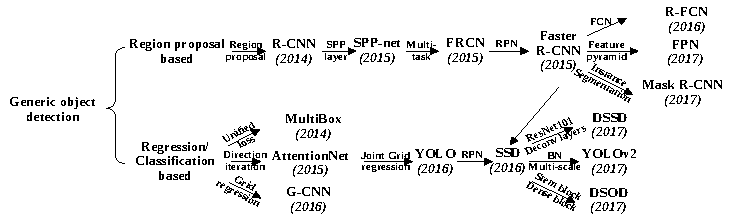
\includegraphics[widht=\textwidth]{figures/deep_roadmap.pdf}
  \caption{Small roadmap of different popular solutions up until 2017 \citep{zhao}}
  \label{fig:deep_roadmap}
\end{figure}

\subsubsection{Region Proposal}
The region proposal framework is a two step process. The framework firstly scans an image and then focuses in any regions in the image of interest. As shown in \autoref{fig:deep_roadmap} the R-CNN solution is one of the first in region proposal approach. The design has three stages in the process of object detection. Firstly a region proposal generation, generating 2000 region proposals for each image. Afterwards a \gls{cnn} is applied to extract features from warped or cropped regions, extracting a 4096-dimensional feature vector. From there classification and categorisation is done with pre-trained \gls{svm}s from multiple classes. The final bounding boxes are produced from adjusted scored regions using bounding box regression.

\subsubsection{Regression or Classification framework}
To compete with the time consumption of regional proposal the one-step framework based on global regression/classification is utilised by mapping straight from image pixels to bounding box coordinates and class probabilities.
This is the technique the framework \gls{yolo} applies. \gls{yolo} divides an input image into $S \times S$ grid, each cell is responsible for predicting the object centred in the cell.
The first \gls{yolo} framework has 24 convolutional layers and 2 \gls{fc} layers \citep{zhao}. The second version, referred to as both \gls{yolo}v2 and \gls{yolo}9000, uses the Darknet-19 model, which has 19 convolutional layers and 5 maxpooling layers. It is based on the Googlenet architecture \citep{Redmon2016}. At the point of deployment this framework has state of the art performance. The third iteration of the framework \gls{yolo}v3 with an update of the Darknet architecture increasing the size from 19 convolutional layers to 53. The newest \gls{yolo} framework is from early 2018 and is still one of the best in its category. In precision \cite{Redmon2018} states the framework does not perform as well as RetinaNet, but the speed of the framework is faster. \gls{yolo} is fast and lightweight enough to run in real time. It is mostly trained on the COCO and VOC datasets \citep{Redmon2018}.

%\graphicspath{{figures/analysis/}}
\chapter{Analysis}\label{ch:analysis}

%\chapter{Problem Statement}

\chapter{Project Specification}\label{ch:projecspec}\glsresetall
This chapter specifies the scope of the project. It outlines and delimits the goals for the work conducted, as well as setting the requirements for the solutions implemented during the project work. 

%\graphicspath{{figures/design/}}
\chapter{Design}\label{ch:design}


\chapter{Implementation}\label{ch:implementation}\glsresetall
Based on \autoref{ch:projectspec}, \nameref{ch:projectspec}, a number of tasks has been set. This chapter clarifies the work done and solutions found to complete the tasks.

\section{Object Detection and Tracking}
As stated in \autoref{sec:main_task} the main task got scaled down due to the amount of other work needed done. Instead of being able to do 6 \gls{dof} object pose tracking of known objects using 3D cameras (for robotic picking of groceries), the first steps of the object pose tracking became essential for showing potential in the idea. 

Instead finding an already working solution of object detection and grasping point estimation and showing a real time object detection solution for groceries became the goals.

\subsection{Grasping Point Estimation}
\cite{Dexnet3} has developed a grasping planning network called Dex-Net. This project was chosen as a viable solution to object grasp planning. This is done over several generations and has two different grasping methods. Both a parallel gripper and suction based end-effectors.

Both implementations of Dex-Net 2.0 and 3.0 are trained using a synthetic dataset of point clods which include grasps and some metrics for grasping quality, either for a parallel gripper or a pneumatic suction cup. This has been modelled for the end-effector in each generation.

The network trained is the \gls{gqcnn} also designed by \cite{Mahler2017}. The network is able to estimate the highest quality grasping point for both end-effectors. The Dex-Net 2.0 is 93\% successful on objects in training and achieves 99\% on a dataset of 40 household objects \citep{Mahler2017}. The Dex-Net 3.0 has three different categories of objects; Basic (prismatic or cylindrical), Typical (more complex geometry), and Adversarial (with few available suction-grasp points) and achieves success rates of 98\%, 82\%, and 58\% respectively. When training with the adversarial objects only, they reach a success rate of 81\%. These objects are shown in \autoref{fig:dexnet3} with the performances of on the different objects.

\subsection{Real Time Object Detection}
The solution needs to be real time, to show the potential of the implementation, for that reason \gls{yolo} is chosen as the model to implement, since it is able to run real time. Opposite to \autoref{sec:yolo_tens} there is no requirement to use Tensorflow, instead a GitHub repository of the \gls{yolo}v3 network is used. \gls{yolo} uses C and CUDA for training neural networks \citep{Redmon2018}. With CUDA the program is able to utilise an Nvidia GPU to drastically lower the training opposed to using just the CPU.

\subsubsection{You Only Look Once}
The implementation of \gls{yolo}v3 used is a forked repository of the Darknet created by Joseph Redmon but with an extended Readme easing insight into training other datasets than the ones included in the repository. Darknet originally uses another annotation than both the COCO and VOC dataset, by using a \lstinline|txt| file for each image in the chosen dataset. An annotation file consists of a line for each new object in the image, with four floats afterwards between 0 and 1 relative to width and height of image in the order: \lstinline|<x_center> <y_center> <width> <height>|.

\subsubsection{Database}
The database used for this is "\gls{d2s}" by \cite{d2s}. This dataset contains 60 different groceries with pixel-wise labels of all object instances. Objects are placed in a setting to resemble a real world setting of an automatic checkout. Each object is featured in several positions and three different lightings of each angle. The setup, lightings and different backgrounds are shown in \autoref{fig:d2s_setup}. The different backgrounds are only used for testing.

\begin{figure}[H]
	\centering
	\includegraphics[width=0.8\textwidth]{figures/d2s_setup}
	\caption{\gls{d2s} image acquisition setup and different lighting settings and the different backgrounds used}
	\label{fig:d2s_setup}
\end{figure}

\subsubsection{Training}
Before training, the data and network cfg need preparation to fit the new data properly. This is due to the network design towards another dataset and annotations for the dataset are not in the right format.\\

The annotations from the \gls{d2s} dataset are written in a json file and needs conversion. This conversion is done using a python script to analyse the json file and write the new files. The script is shown in \autoref{sec:json_conversion} in the appendix.

Besides the annotations, the network needs a file path to every training and test image from the root of the executable program.\\

In the cfg for the network it is important to change the amount of classes to the amount in the custom dataset i.e. 60. When changing the amount of classes, recalculating the anchors can boost performance. A script for this is included in the repository and only needs the image paths file.
The filters in the cfg also need changing as these are set based on the amount of classes in the dataset, these should be: $\text{filters} = (60_{classes} + 5) \cdot 3 = \underline{195}$.\\

To increase accuracy the network is trained with pre-trained weights from the Darknet website for \gls{yolo}v3. The network is trained with a batch size of 64 and a learning rate at $10^{-3}$ for $83\,000$ iterations.

\subsection{Results}
After $83\,000$ iterations the network started to be unstable and was stopped at an average loss of $ 0.7171 $. The loss curve for the training is shown in \autoref{fig:chart}.

\begin{figure}[H]
	\centering
	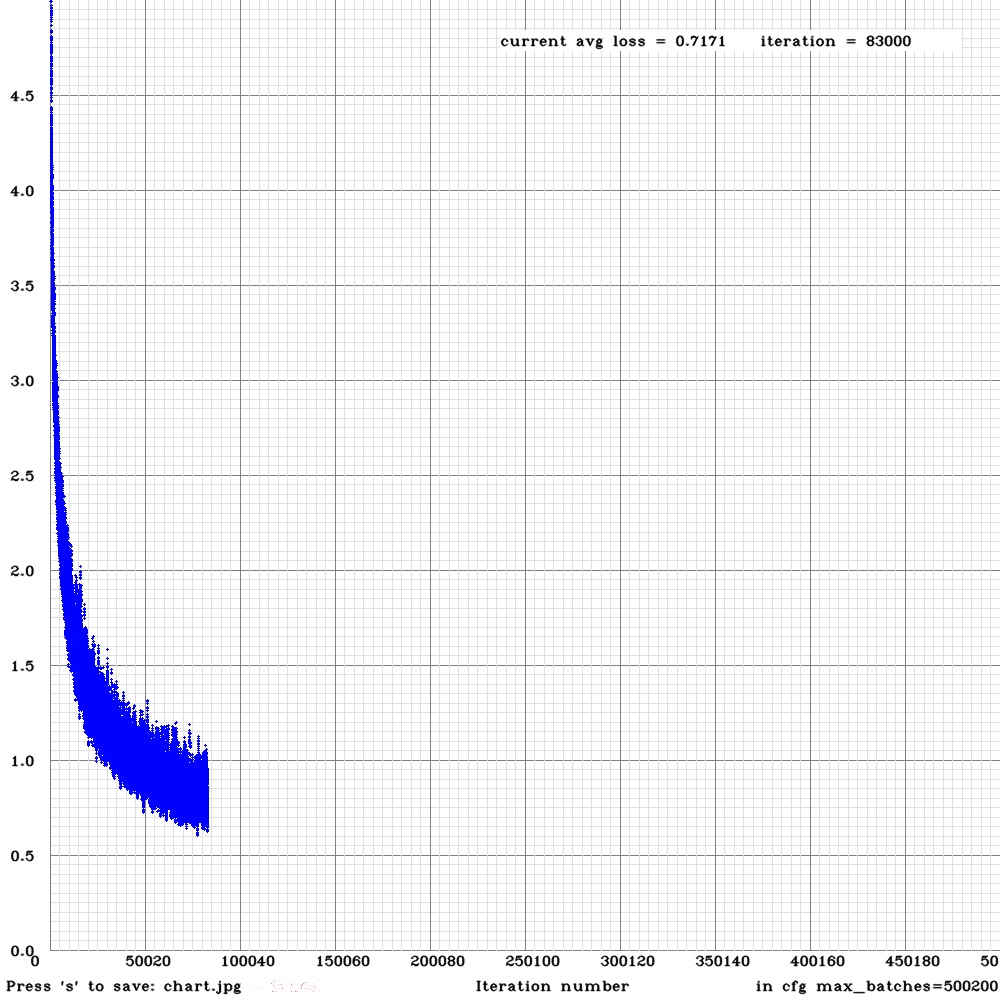
\includegraphics[width=0.6\textwidth]{figures/chart}
	\caption{Loss curve for training Darknet for the \gls{d2s} database}
	\label{fig:chart}
\end{figure}

The trained network is then tested on both single testing images to see if it is able to detect objects in those. An example of this is shown in \autoref{fig:combo_predict}.

\begin{figure}[H]
	\centering
	\begin{subfigure}[b]{0.45\textwidth}
		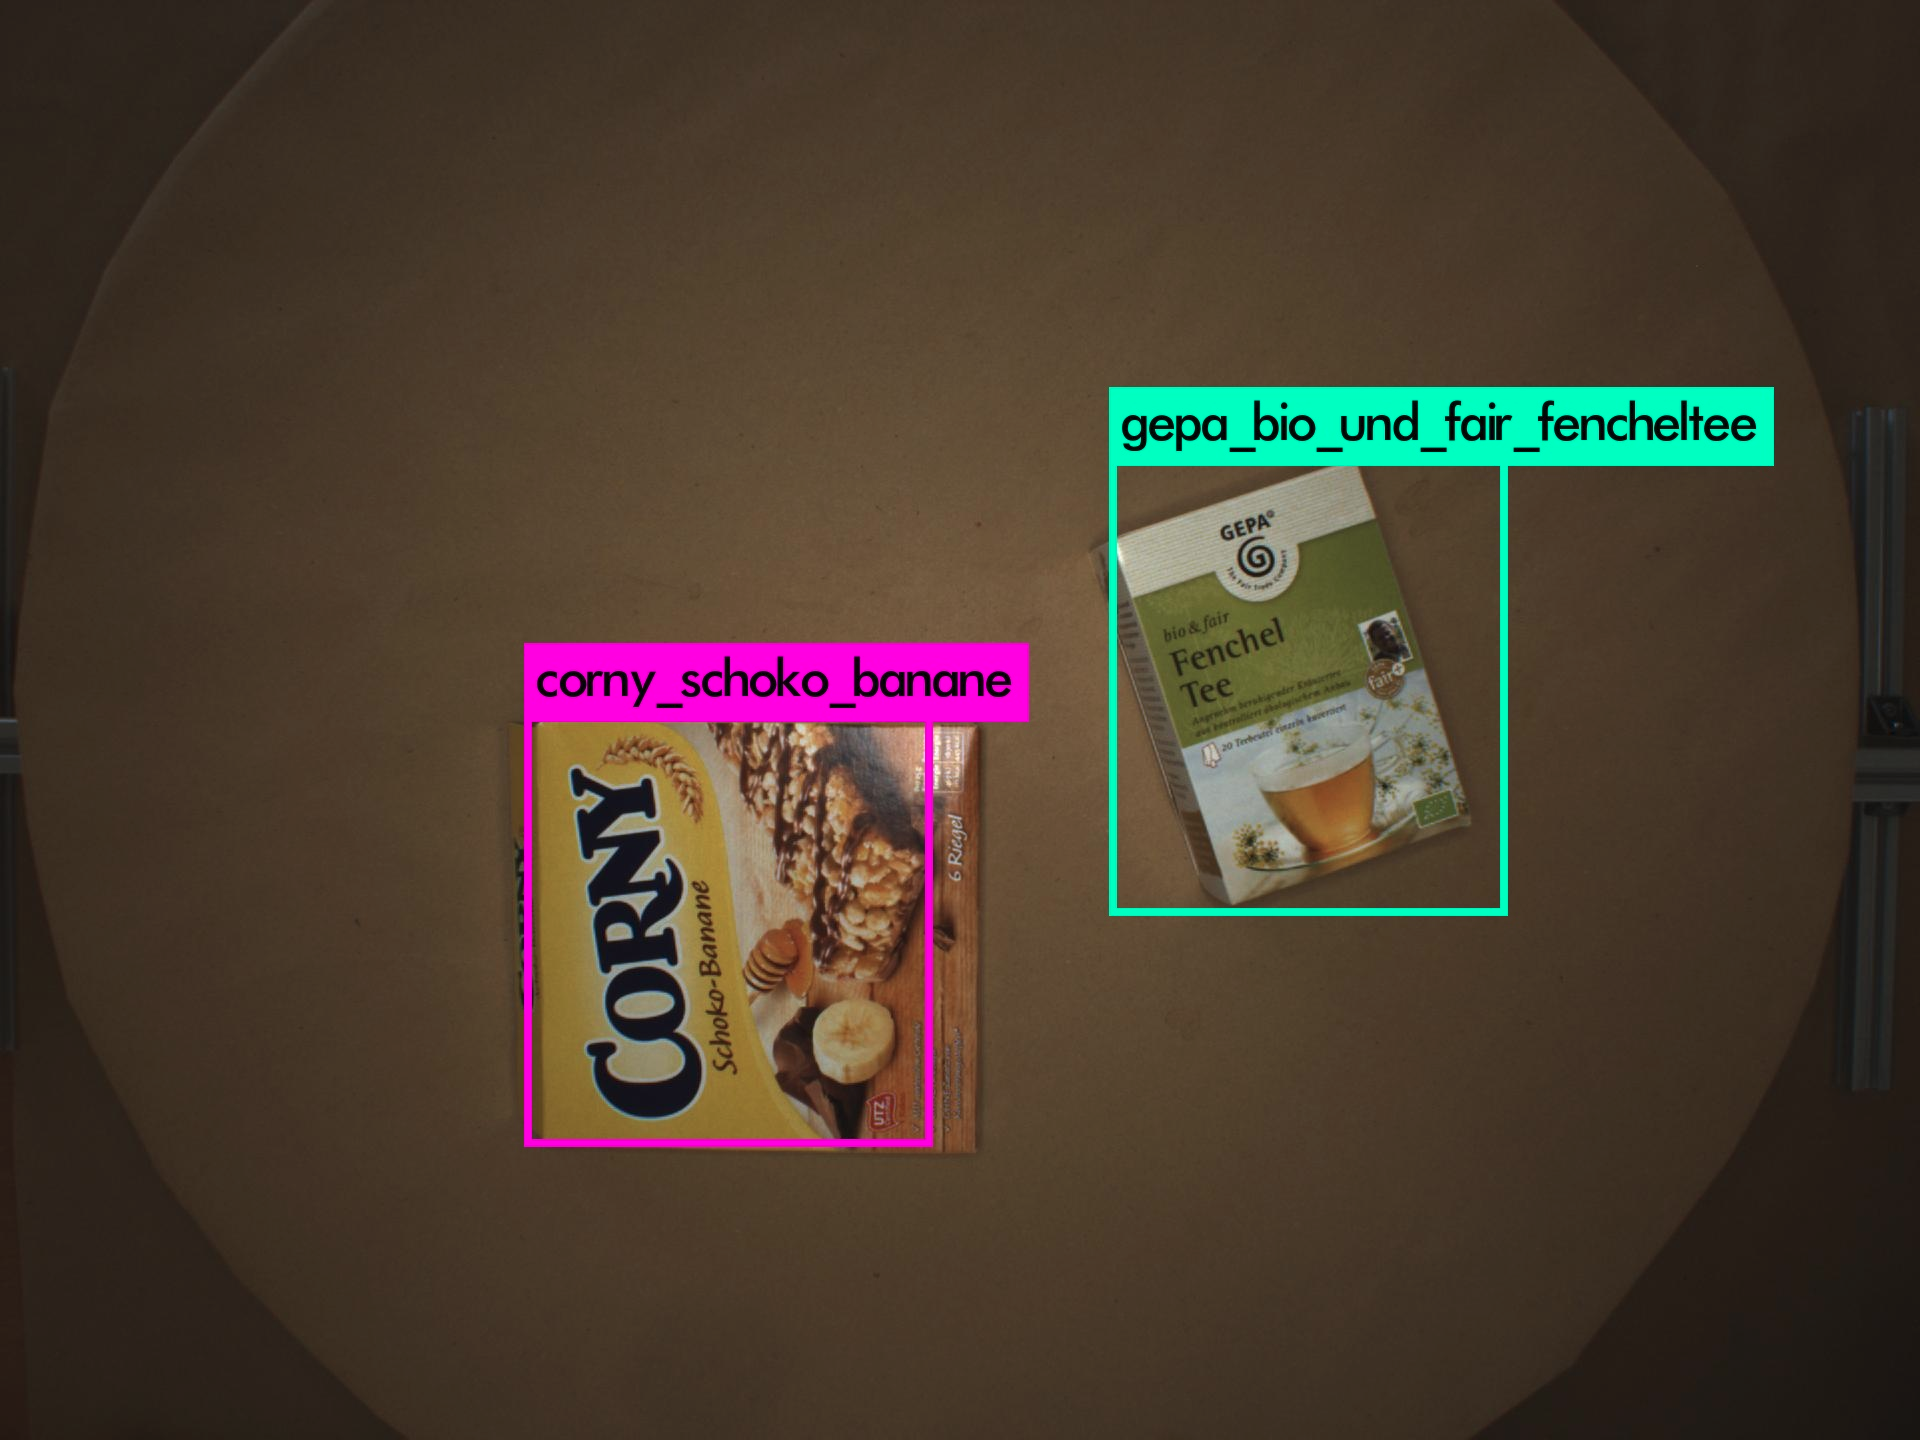
\includegraphics[width=\textwidth]{figures/result_2_obj}
		\caption{Two objects from the \gls{d2s} dataset recognised by the network}
		\label{fig:result_2_obj}
	\end{subfigure}
	~
	\begin{subfigure}[b]{0.45\textwidth}
		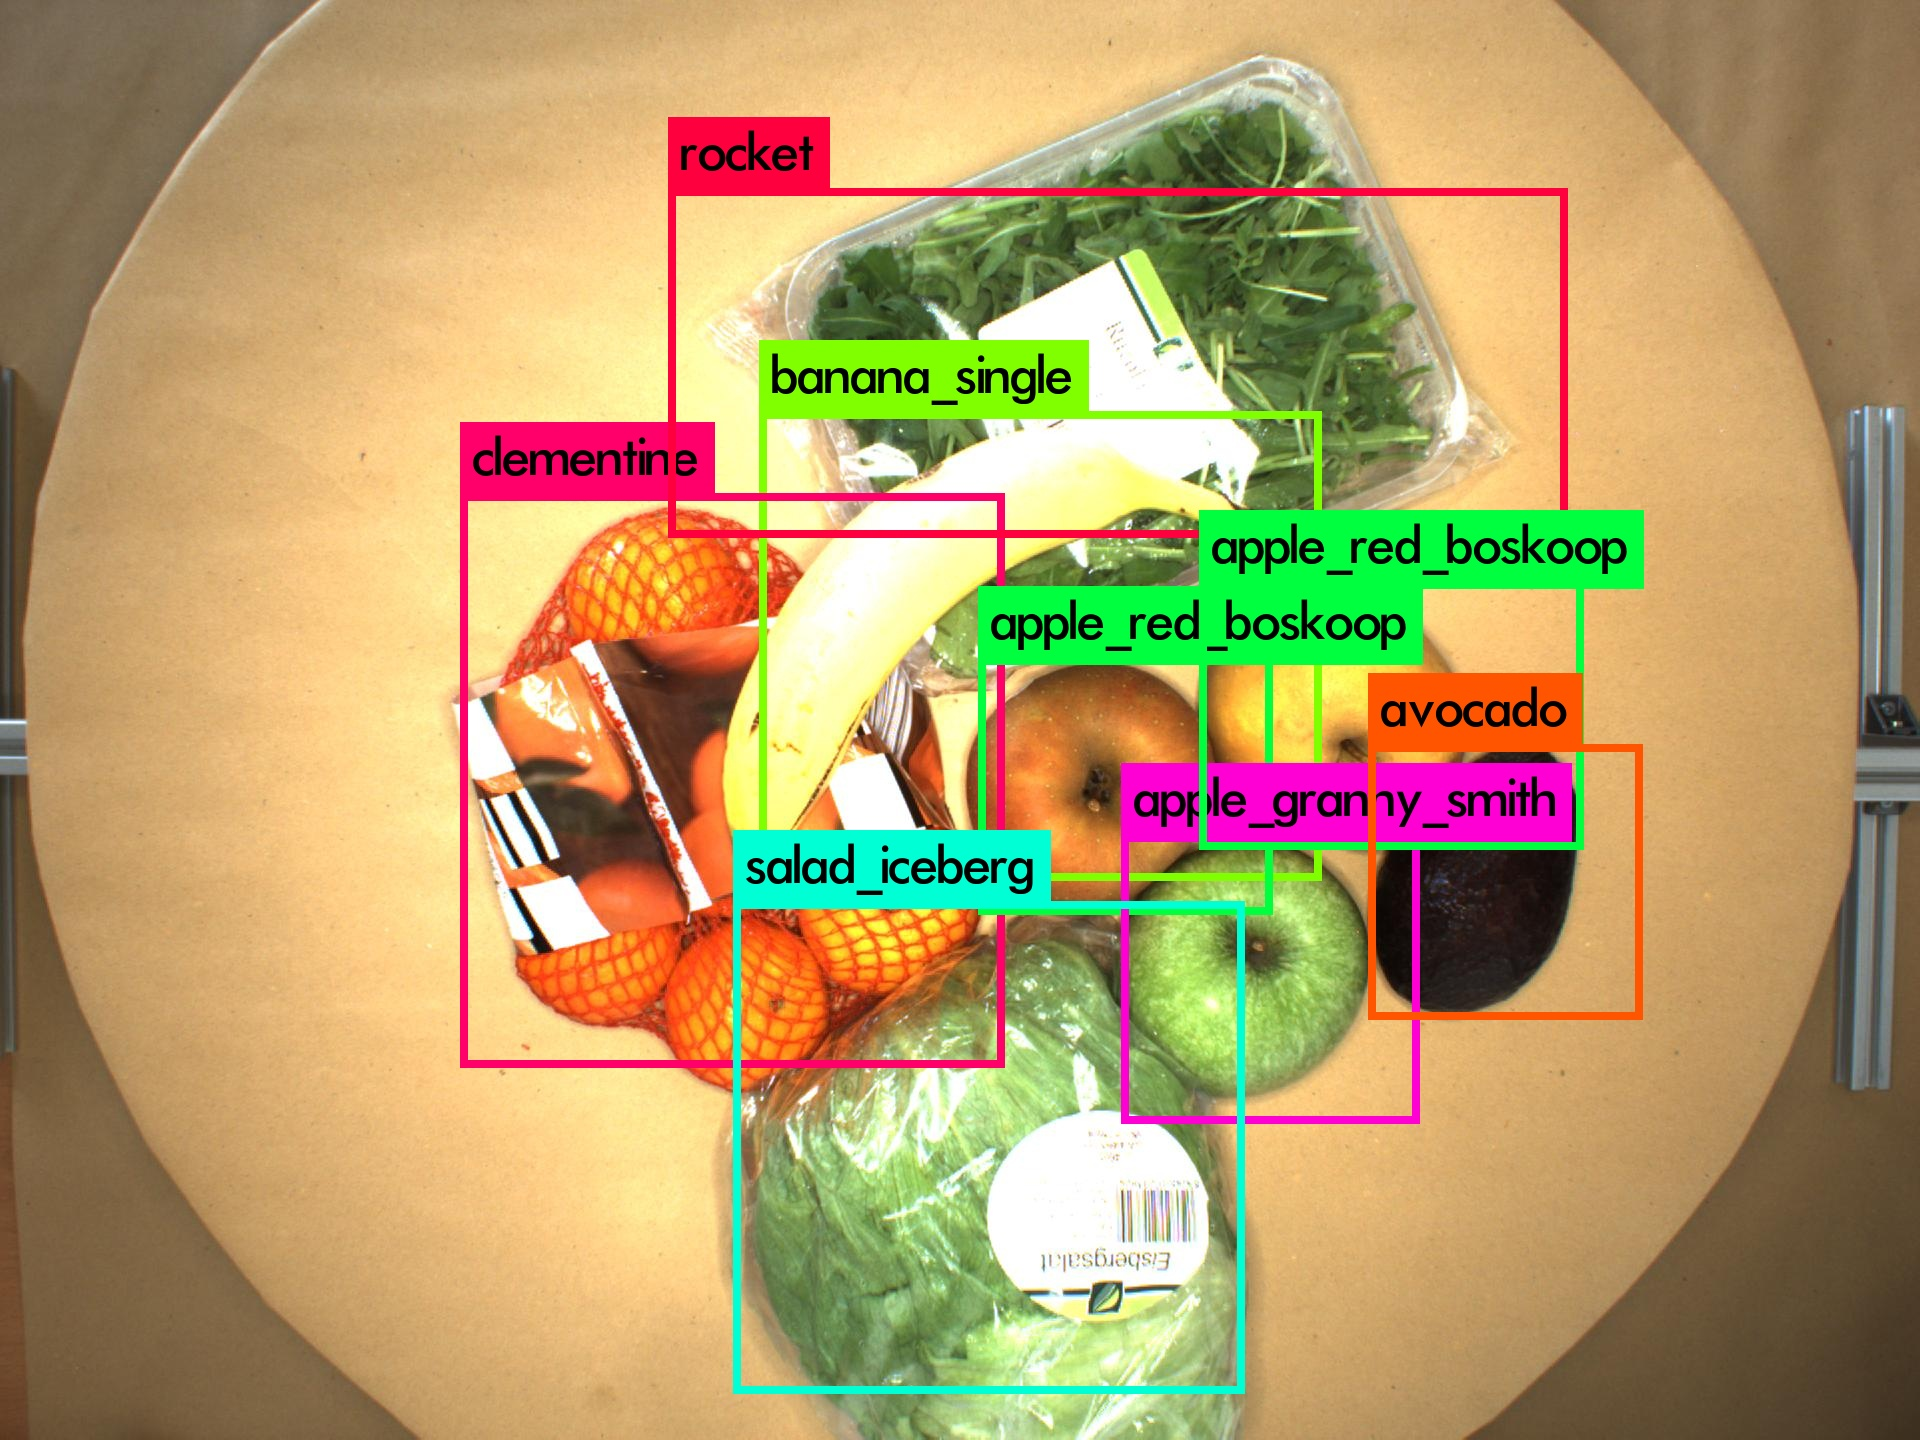
\includegraphics[width=\textwidth]{figures/predictions_mass}
		\caption{Multiple objects from the \gls{d2s} dataset recognised by the network}
		\label{fig:pred_mass}
	\end{subfigure}
	\caption{Single tested images from the \gls{d2s} dataset}
	\label{fig:combo_predict}
\end{figure}

When testing on a home recorded video of different objects the network is having issues recognising objects in the scene. The recorded scene consists of two apples and a banana, which are the only objects resembling objects from the database. It does somewhat recognise the apples and the banana at points, but the certainty varies. It also has some false positives during the test video. While analysing the video, the certainties are output in the terminal running the detection, a dump of some of this output is found in an attached zip file with the report with the name \lstinline|d2s_dump.txt|. 

Screenshots of the video with both false positives and true positives are shown in \autoref{fig:yolo_video}. Due to an offset of the bounding boxes, the corner of a box is marking the centre of the object. This issue only occurs in the video test and not in the single images. As the terminal output is limited to a certain amount of lines, not all frames are included in the certainty dump file.
\begin{figure}[H]
	\centering
	\begin{subfigure}[b]{0.48\textwidth}
		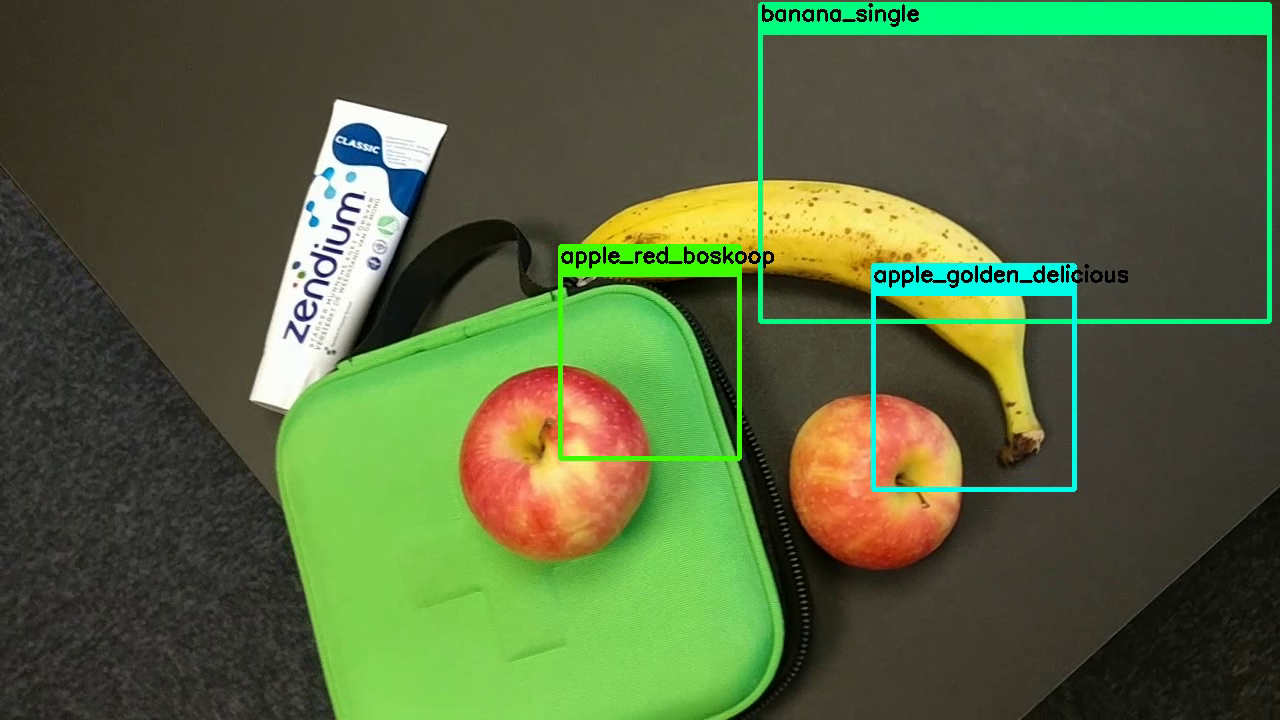
\includegraphics[width=\textwidth]{figures/yolo1}
		\caption{True positives with certainties at:\\ banana_single: 80\%\\ apple_golden_delicious: 28\%\\ apple_red_boskoop: 37\%}
		\label{fig:yolo1}
	\end{subfigure}
	~
	\begin{subfigure}[b]{0.48\textwidth}
		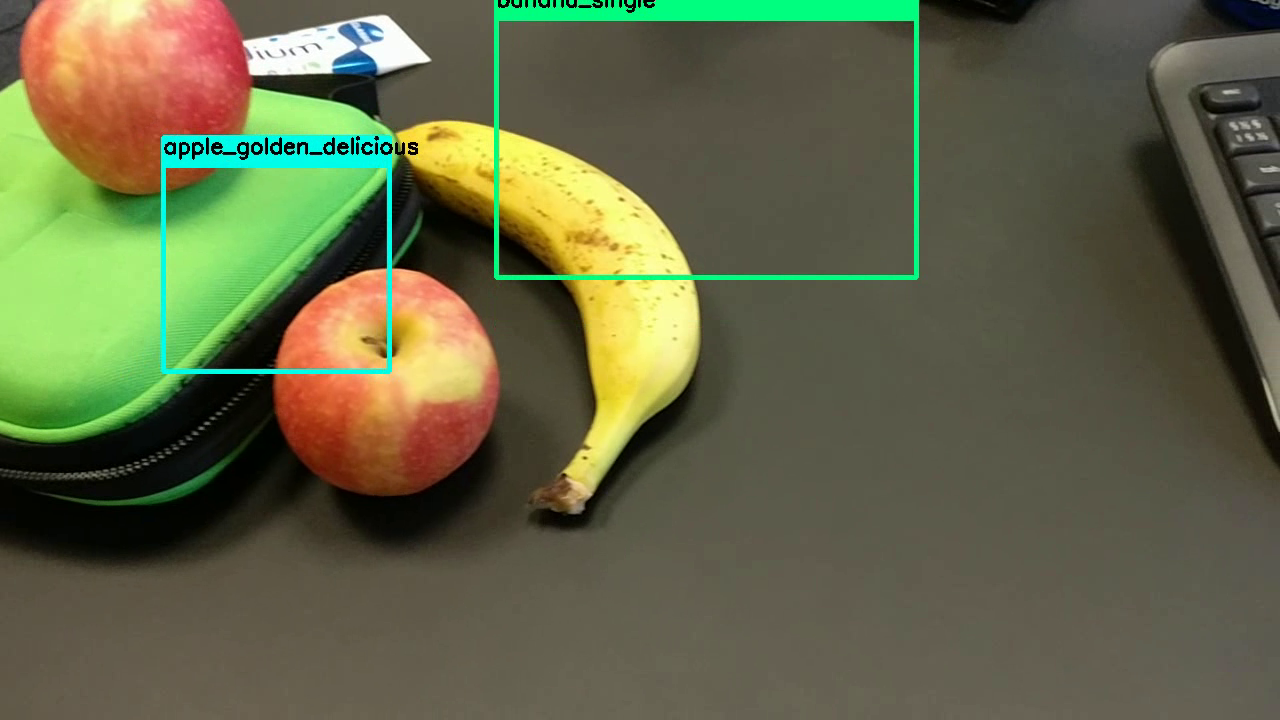
\includegraphics[width=\textwidth]{figures/yolo2}
		\caption{True positives with certainties:\\ banana_single: 47\%\\
			apple_golden_delicious: 85\%\\}
		\label{fig:yolo2}
	\end{subfigure}

	\begin{subfigure}[b]{0.48\textwidth}
		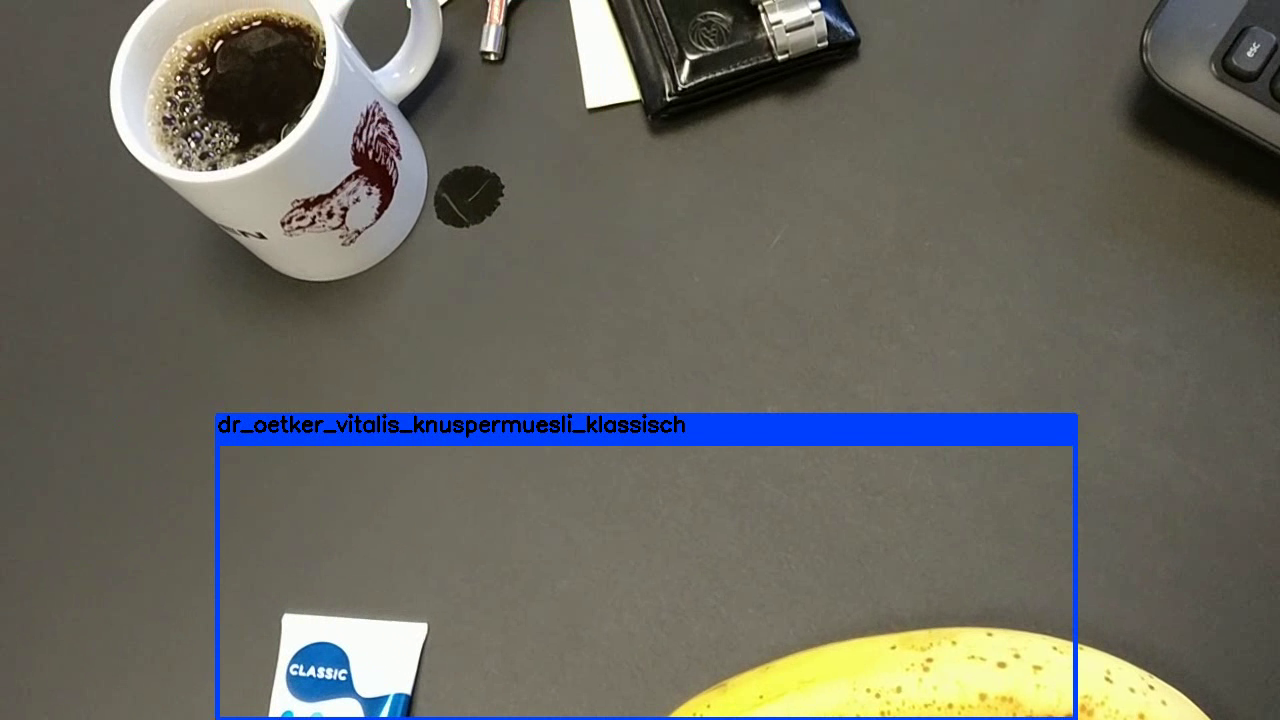
\includegraphics[width=\textwidth]{figures/yolo3}
		\caption{False positive with certainty: dr_oetker_vitalis_knuspermuesli_klassisch: 32\%}
		\label{fig:yolo3}
	\end{subfigure}
	~
	\begin{subfigure}[b]{0.48\textwidth}
		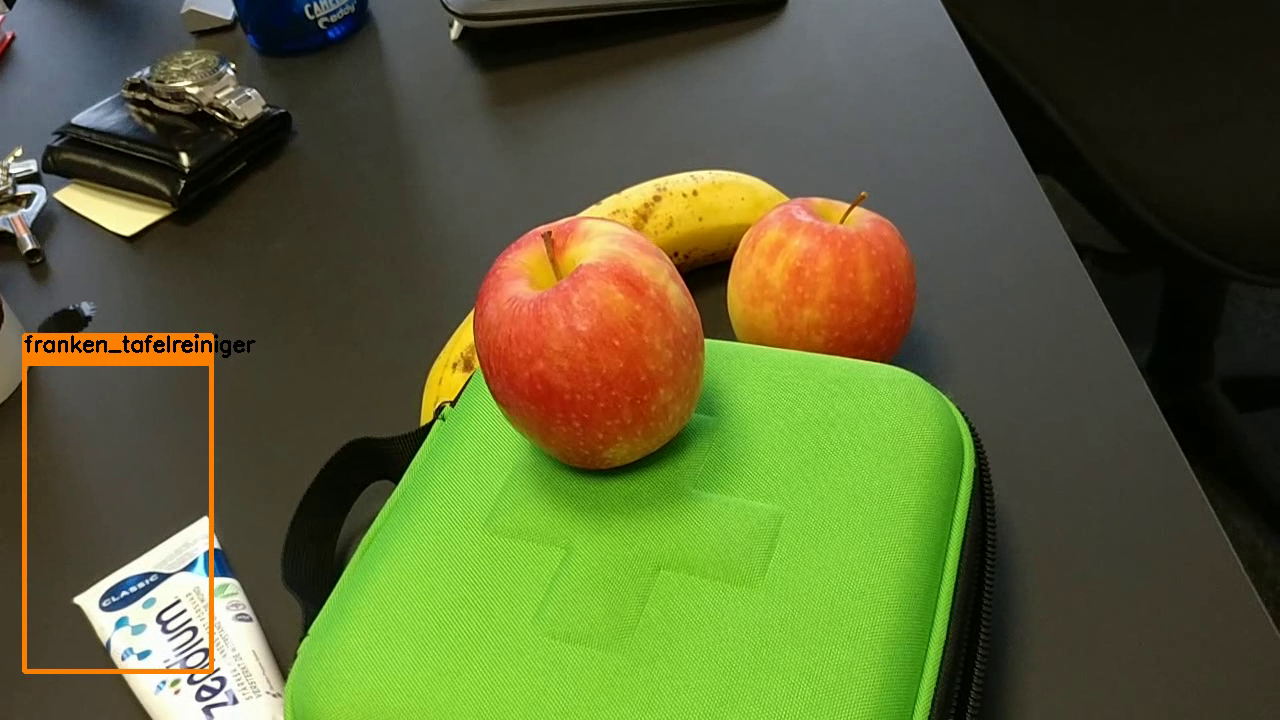
\includegraphics[width=\textwidth]{figures/yolo4}
		\caption{False positive with certainty: franken_tafelreiniger: 55\%\\}
		\label{fig:yolo4}
	\end{subfigure}
\caption{Screenshots of the video with both false positives and true positives}
\label{fig:yolo_video}
\end{figure}

An overview of the precision on each object class is shown in \autoref{ch:D2S_prec}. This also shown the mean average precision is $ 48.17 \% $.

The test video is also found in the attached zip file with the report, under the name \lstinline|darknet_test_video.avi|.

\section{YOLOv3 Tensorflow Implementation}\label{sec:yolo_tens}
As the solution is supposed to work real time, \gls{yolo} was chosen as the desired solution, but also because the CTO had had \gls{yolo} running before using the standard setup of the Darknet running in C trained on the COCO dataset.

Because of the desire to have it running on Tensorflow another version of Darknet is needed, as Tensorflow works with Python and not C. 
Given previous experience with Keras, a solution build upon this is preferred as this will ease the understanding of the implementation and make potential changes to the network easier to do.

\subsection{Keras YOLO3}\label{sec:kerasyolo}
The Keras implementation is found on GitHub and is made for \gls{yolo}v3. It is based on another repository made with the \gls{yolo}v2 Darknet version, which is a smaller network, but also with a general lower precision \citep{Redmon2016, Redmon2018}. The repository is found at: \url{https://github.com/qqwweee/keras-yolo3}.

This is a conversion of the network design to a Keras implementation. It employs the annotation layout of one row for each image in a text file with every bounding box in the image separated with spaces:\\

\noindent Row format: \lstinline{image_file_path box1 box2 ... boxN}, and\\ Box format: \lstinline{x_min,y_min,x_max,y_max,class_id}.

\subsection{Dataset}
It was requested, that the object detection was trained to recognise some industrial objects such as screws, electric fuses for a fuse box and extension boxes. The dataset chosen is "T-LESS: An RGB-D Dataset for 6D Pose Estimation of Texture-less Objects" made by \cite{tless}. 

As stated in the title of the article for the dataset, the dataset is a an \gls{rgbd} dataset. As \gls{yolo} only works with one type of images only the RGB images are used.

\subsection{Training}
The training is done by running a Python script with Tensorflow activated, to enable GPU processing, which launches the training. Before training, the data needs to be prepared, as the annotation of the dataset differs from the on the network uses.
\subsubsection{Data Preparation}
As the annotations from the T-Less dataset is written in an XML file format with a file for each image of each object, a conversion is necessary. This is done with a small Python script converting to the annotation style mentioned in \autoref{sec:kerasyolo}. The script is shown in \autoref{sec:tless_conv} in the appendix.

\subsubsection{Training Setup}
The setup of the network is including a \lstinline{ReduceLROnPlateau} function, which reduces the learning rate when a metric has stopped improving. Another callback function included is \lstinline{EarlyStopping} which stops the training when a certain set improvement is not met for a specified amount of iterations.

\gls{yolo}v3 uses the Darknet-53 \gls{cnn} which has 53 convolutional layers. This is also shown in \autoref{fig:darknet53}. The last \gls{fc} layer has been changed from 1000 classes to 30, as this is the amount of classes included in the T-Less dataset. The training is done with pre-trained weights from the Darknet training with the COCO dataset.

\begin{figure}[H]
	\centering
	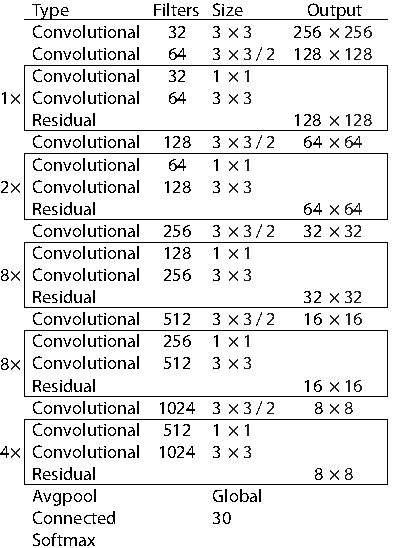
\includegraphics[width=0.45\textwidth]{figures/darknet53}
	\caption{Overview of Darknet-53, the \gls{cnn} used with \gls{yolo}v3 \citep{Redmon2018}}
	\label{fig:darknet53}
\end{figure}

For training, the optimiser Adam is used, first with a learning rate of $ 10^{-3} $ if more training is needed after 50 epochs and the learning rate has not been lowered, it is lowered to $ 10^{-4} $, and with a batch size of 32. 

\subsection{Results}
Due to a limited amount of time and objects resembling the objects in the dataset, the testing video used for this network only included one item from the T-Less dataset, an electric fuse. The fuse is filmed in an office setting with a keyboard, laptop, monitor visible in the video as well. This object was chosen as it was easy to find in many situations and places, which meant it might also be possible to find one at the Robot Union event, which the demo was for.

Unfortunately, the precision was not high enough to show a demo at the event. As shown in \autoref{fig:tens_accuracy}, there was a lot of false positives in the testing and low accuracy when detecting the desired object. In the video, the object \textit{03} is the fuse.

\begin{figure}[H]
	\centering
	\begin{subfigure}[b]{0.48\textwidth}
		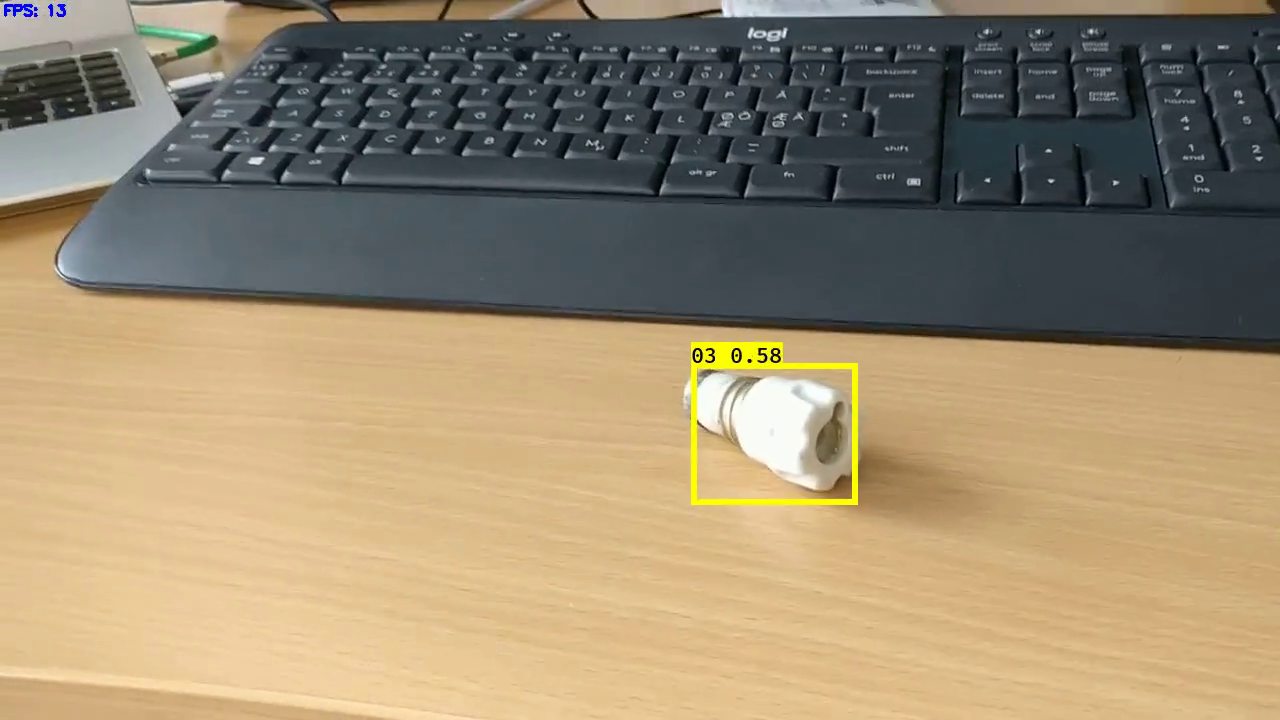
\includegraphics[width=\textwidth]{figures/tens1}
		\caption{True positive, fuse detected with 58\% certainty}
		\label{fig:tens1}
	\end{subfigure}
	~
	\begin{subfigure}[b]{0.48\textwidth}
		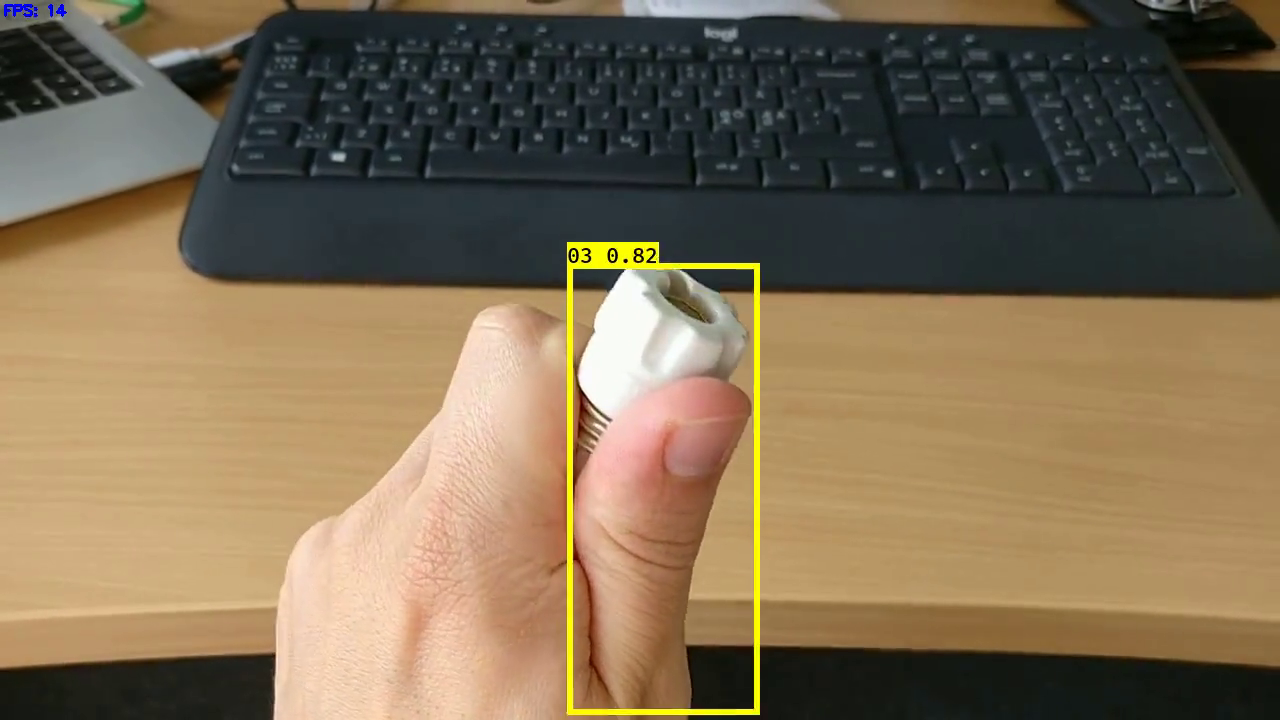
\includegraphics[width=\textwidth]{figures/tens2}
		\caption{True positive with occlusion, fuse detected with 82\% certainty}
		\label{fig:tens2}
	\end{subfigure}

	\begin{subfigure}[b]{0.48\textwidth}
	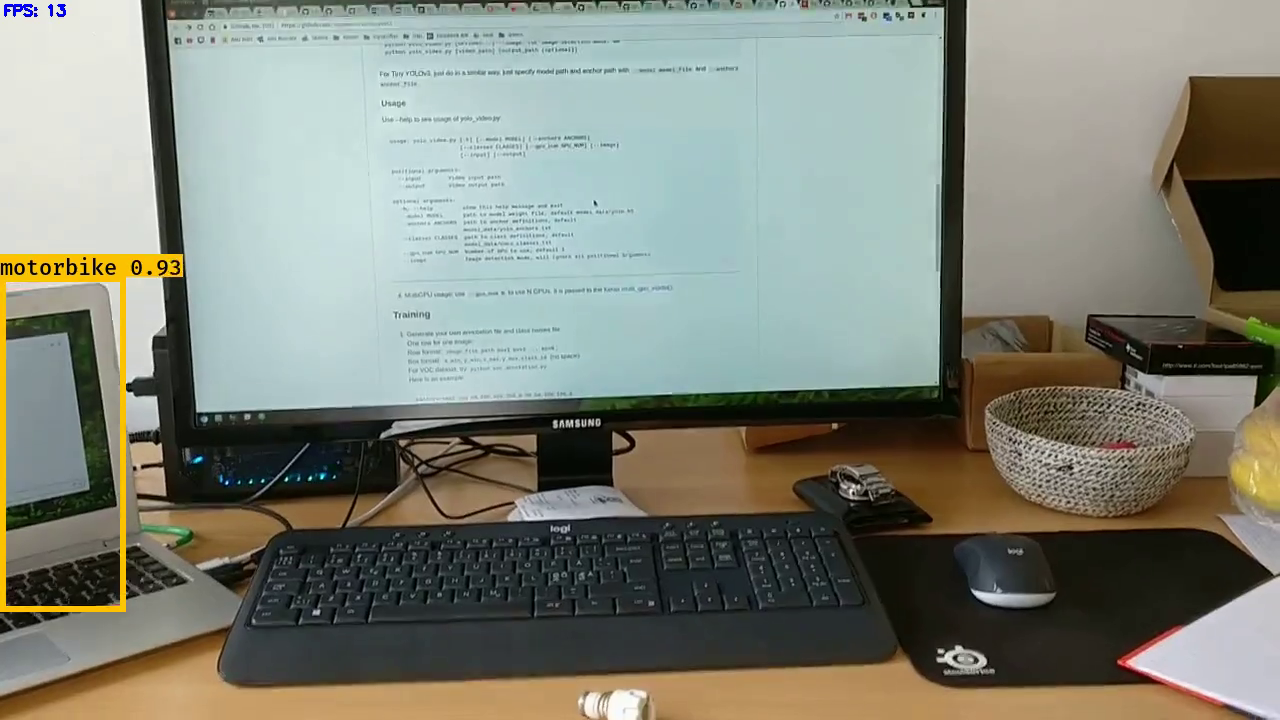
\includegraphics[width=\textwidth]{figures/tens3}
	\caption{False positive detection of a motorbike}
	\label{fig:tens3}
	\end{subfigure}
	~
	\begin{subfigure}[b]{0.48\textwidth}
		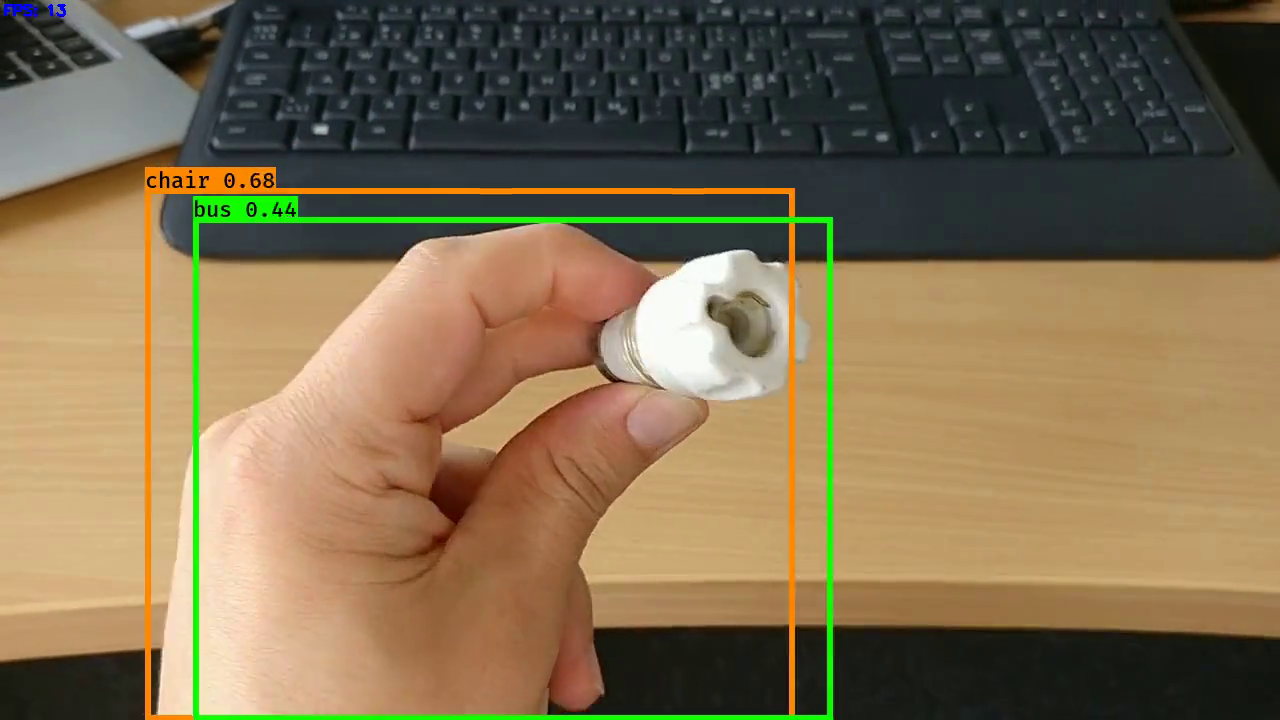
\includegraphics[width=\textwidth]{figures/tens4}
		\caption{False positive detection of chair and bus}
		\label{fig:tens4}
	\end{subfigure}
	\caption{Video test results for the \gls{yolo}v3 network trained on the T-Less dataset}
	\label{fig:tens_accuracy}
\end{figure} 

\section{Matrix Storage}
This task was intended as an on stream process, storing the video data before compressing as matrices to a file, to automate testing of the camera compression algorithm. At the point of development, the core solution of the pipeline was written in C++ and not the final GStreamer solution implemented for the video streaming solution.

This task required some insight into the meta solution of the pipeline already written and understanding of the code. The code had several dependencies and required some extra functionality in order to generate the data as wanted.

Before reaching a solution to the task, another solution for the pipeline was made, and therefore made the task obsolete.

\section{GStreamer Pipeline Configuration}\label{sec:gstream_design}
The pipeline configuration consists of several smaller tasks within the same \gls{gstapp}. In total it has three functions:

\begin{itemize}
	\item Receive RTP packages and store them in the desired destination
	\item Receive RTP packages, decompress, and play them back to the user
	\item Decompress the video data and play it for the user
\end{itemize}

The source for the RTP packages is a UDP source, which means an IP and a port needs to be set to receive the packages. When testing, the IP is localhost i.e. \lstinline|127.0.0.1|, and the port depends on which video stream the user wants to receive, as there are both an id stream, a depth video stream and a colour video stream. These are either \lstinline|9000|, \lstinline|9001|, or \lstinline|9002|. It is important to set the same ports on the sender side in order to receive data.

The data received is payloaded and has h265 encoding which needs de-payloading and decoding before storing to file or playing back. 

When differing between storing and streaming to a video player, it is only one command in difference. It is either \lstinline|filesink| and a path to destination for storing or \lstinline|fpsdisplaysink| to play back the video.

Besides these settings, it is important to match \textit{caps} which are video settings set from the sender side, and must also be et on the receiver side. These depend on the file type. An example of a GStreamer command to receive and store a video file is:

\noindent\textbf{\lstinline|gst-launch-1.0 videotestsrc num-buffers=100 ! x265enc tune=zerolatency ! video/x-h265, stream-format=byte-stream,alignment=au ! filesink location=h265.pay|}

\section{Docker Set Up}
The docker set up was to be able to test the \gls{gstapp} described in \autoref{sec:gstream_design}, by having it running in a docker container on an Nvidia TX2.

Due to Docker being a new area, learning of Docker composing was necessary, which was also a goal in the task more than getting the test scenario running. Training and learning was done using the website \url{https://training.play-with-docker.com/}.

The set up was to be build upon a barebone ROS Balena image, which had been build before. This meant the docker still needed some Catkin set up and enabling for building with Meson and Conan, and then calling the build command in the docker, and the \gls{gstapp} would be ready to launch. 

With a sender in one docker and the receiver in another the testing of the communication is done. The majority of the time spent on the task was learning how Docker works and not the design of the docker file written.
\chapter{Evaluation}

\chapter{Conclusion}\label{ch:conclusion}\glsresetall
During the internship the main task has been to develop a system with;\\

\textit{6 \gls{dof} object pose tracking of known objects using 3D cameras (for robotic picking of groceries).}\\

Due to time constraints this main task was decreased to show the possibility of implementing real time object detection with a grocery dataset and showing a solution of grasping estimation on objects with deep learning.

The Dex-Net implementations show that it is possible to estimate grasping points of objects when the right model is applied to a big dataset, even with synthetic data. The robot is able to evaluate the \gls{rgbd} input data after training and can estimate a successful grasping point with high precision.

The real time object detection is made using \gls{yolo}v3, as this network is known for being a fast, lightweight network. The dataset used is a grocery dataset with 60 different object classes including annotations. The mean average precision achieved with the network is $ 48.17\% $ on the test images. This precision has proven too low to handle the test video, showing a lot of false positives and in general low precision on each object class, as seen in \autoref{ch:D2S_prec}. A proposed solution to increase precision, is to add more data by augmenting the training images with several different methods.

Being in a company meant several tasks instead of just one project. The other tasks lead to learning new skills in programming and IT knowledge. The tasks was assigned due to a deadline, which meant they had highest priority, taking away time from the main project.

Due to being the sole employee working with computer vision, discussing solutions was not always possible because of the lack of insight in the subject. 

The internship has shown how it is being a part of a company and has given some experience in working with people outside of the university programme. It has also been testing the various skills learned and made for improvement in several subjects. It has furthermore given inspiration to future plans after the university.
\chapter{Future Work}


% For use if report is split up in parts
\bookmarksetup{startatroot}% Goto root of Table of Contents
\addtocontents{toc}{\bigskip}% Add space before next item in Table of Contents

% Appearance of the bibliography
\iflanguage{english}{%
\bibliographystyle{setup/plainnat_en}%
}{%
\bibliographystyle{setup/plainnat_dk}%
}
\label{LastPage}


\bibliography{bib/library.bib}
\label{bib:mybiblio}




%\setlength{\chapnumb}{2cm} % Ændrer længden på stregen under kapiteloverskriften så den passer til bilag
\appendix % Start of appendix
\addtocontents{toc}{\protect\setcounter{tocdepth}{0}}


\end{document}
